\chapter{Experimentos}

\section{Implementación}
\label{section4:implementation}
\subsection{Entorno de desarrollo}
\subsubsection{Software}
Debido a su amplio uso en el ámbito de la IA y la Ciencia de Datos, y siendo el lenguaje de programación utilizado para la implementación de ExMeshCNN, este TFM ha sido desarrollado íntegramente en Python 3. Para la construcción de las redes neuronales se ha empleado de forma predominante la librería PyTorch junto con la librería de optimización de parámetros Optuna, complementada por otras bibliotecas ampliamente utilizadas en ML como NumPy, SciPy, Scikit-Learn y Pandas.

Dado que los datos tratados son de naturaleza tridimensional, se ha recurrido extensivamente a herramientas especializadas para la manipulación de mallas 3D. Entre ellas destacan el software de código abierto Blender y su API para Python, así como las librerías PyMeshLab, Trimesh y OpenMesh.

La gestión del control de versiones se ha llevado a cabo mediante Git y GitHub. Por otro lado, la gestión de dependencias del entorno Python se ha realizado mediante un entorno virtual (\textit{Virtual Environment}) específico para este proyecto.

El código desarrollado en el presente trabajo se encuentra disponible en el siguiente repositorio: \url{https://github.com/RhinoBlindado/datcom-tfm}.

\subsubsection{Hardware}
La ejecución de este TFM se ha llevado a cabo en dos entornos diferenciados: uno local y otro remoto.

El entorno local consistió en un ordenador portátil Asus FX505DT equipado con un procesador AMD Ryzen 7 3750H, 16 GB de memoria RAM y una GPU Nvidia GeForce GTX 1650 con 4 GB de VRAM. En este entorno se desarrolló el código fuente, así como las tareas de preprocesamiento de datos y pruebas a pequeña escala, dada la capacidad limitada de procesamiento gráfico.

El entorno remoto correspondió al clúster de servidores GPU de la Universidad de Granada, denominado NGPU, ubicado en el CPD Santa Lucía. En particular, se utilizó preferentemente el nodo denominado Talos, que dispone de dos procesadores AMD EPYC 7742, 1 TB de memoria RAM y 8 GPUs Nvidia Tesla A100, cada una con 40 GB de VRAM. En este entorno se ejecutaron la totalidad de los experimentos a gran escala, gestionados mediante acceso remoto vía SSH y utilizando el sistema de planificación de tareas SLURM.

\subsection{Preprocesamiento de datos}
Como se ha mencionado en la Sección \ref{section4:materials}, los datos obtenidos para este proyecto provienen de escaneos en 3D de piezas anatómicas reales digitalizadas usando el escáner Artec Miro que permite captar datos en 3D en una zona de hasta 324 cm$^3$ y escanearlos con una precisión muy alta de hasta 10 micras y una resolución de hasta 0.029 mm \cite{artec_data}. Las mallas generadas a través de estos procesos resultan en geometrías incompletas, degeneradas y con gran variabilidad de resolución. Estos factores impiden su uso directo por el \textit{framework} de ExMeshCNN.

Antes de llevar a cabo los procesos de reparación, remuestreo y reducción de resolución, se consideró necesario unificar la orientación de las muestras, dado que el conjunto de datos incluye tanto pubis izquierdas como derechas. Con el fin de mantener la consistencia geométrica en los datos, se desarrolló un \textit{script} en Blender que aplica el modificador de espejo sobre las mallas 3D correspondientes a las pubis derechas. Este proceso refleja las mallas respecto al eje principal de simetría de la cara anatómica, transformándolas efectivamente en pubis izquierdas. De este modo, se garantiza que todas las muestras procesadas posean una orientación uniforme, realizado con el fin de eliminar posibles fuentes de ruido para el modelo.

\subsubsection{Reparación y remuestreo de datos}
\label{section4:data_repair}

La reparación de las mallas tridimensionales implica tres pasos fundamentales: (1) sellado de los huecos para garantizar que sean estructuras \textit{watertight} (herméticas), (2) eliminación de geometría degenerada, como triángulos solapados, caras conectadas por un único vértice o aristas que se interceptan, y (3) supresión de geometría disconexa perteneciente a componentes menores, generada usualmente por errores en la captura mediante escáner 3D, y que no aporta información relevante.

Para abordar este proceso, se emplearon de forma intensiva las funcionalidades de la API de Blender y de PyMeshLab, desarrollando una serie de \textit{scripts} personalizados para automatizar la limpieza y normalización de las mallas.

En primer lugar, se parte de la malla cruda obtenida del escaneo, denominada \code{raw}. Utilizando PyMeshLab, se aplican métodos predefinidos para eliminar componentes desconectadas, caras duplicadas y geometría \textit{non-manifold}. El resultado de esta etapa es una malla depurada, sin degeneraciones geométricas, denominada \code{raw_clean}.

Sin embargo, esta malla aún puede contener huecos, por lo que no está lista para ser procesada por ExMeshCNN. El cierre de huecos en mallas 3D es una tarea compleja, pero puede abordarse de forma eficaz mediante una técnica alternativa: el remuestreo. Esta técnica genera una nueva topología manteniendo la forma superficial original de la malla. El proceso se basa en una aproximación iterativa mediante vóxeles, que reconstruye la superficie al tiempo que genera la conectividad necesaria para cerrar los huecos.

Para ello, se empleó Blender, que dispone de un operador de remuestreo robusto. Se desarrolló un segundo script que toma como entrada la malla \code{raw_clean} y aplica el operador de remuestreo en modo \code{SHARP}, con una profundidad del árbol octal de 10 (para preservar la fidelidad geométrica) y una escala de 1. El resultado es una malla libre de huecos, aunque este proceso puede reintroducir geometría \textit{non-manifold}.

Por lo tanto, en el mismo script se implementó un procedimiento iterativo para eliminar dicha geometría no válida. Este procedimiento incluye:

\begin{enumerate}
    \item Selección y eliminación de vértices \textit{non-manifold} duplicados.
    \item Nueva selección de vértices \textit{non-manifold} y colapso de aristas entre los vértices afectados.
    \item Nueva selección y eliminación directa de todos los vértices \textit{non-manifold}.
\end{enumerate}
Este ciclo entero se repite hasta que no se detectan más vértices \textit{non-manifold} al final de proceso. Se comprobó empíricamente que este procedimiento converge, generando finalmente mallas completamente selladas y con una topología coherente. A las mallas resultantes se les denomina \code{clean_remesh}.

\subsubsection{Reducción de resolución}
\label{section4:data_reduction}
Una vez obtenidas las mallas \code{clean_remesh}, que presentan una geometría adecuada y sin defectos topológicos, persiste una variabilidad importante: el número de triángulos varía entre mallas. Para normalizar esta característica, se diseñaron dos procesos distintos que permiten obtener versiones reducidas y estandarizadas de las mallas, generando dos conjuntos de datos derivados a partir de cada una.

En el primer proceso, se aplica una reducción global de resolución a la malla \code{clean_remesh} mediante colapso de aristas. Esta técnica, implementada en un script de Blender, permite reducir de forma progresiva el número de triángulos, preservando en la medida de lo posible la topología general y los detalles relevantes. El resultado son mallas con un número fijo de triángulos especificado por el usuario. Estas versiones se nombran como \code{clean_remesh_<x>K}, donde \code{<x>} representa la cantidad de triángulos en miles. Por ejemplo, una malla con 50,000 triángulos tendría el sufijo \code{clean_remesh_50K}.

No obstante, esta reducción uniforme afecta por igual a todas las regiones de la malla, incluyendo zonas anatómicamente poco relevantes para el análisis forense, como la parte posterior del hueso. Para maximizar la preservación de detalles en las regiones de interés, se implementó un segundo proceso complementario. Este consiste en realizar un recorte anatómico antes de la reducción de resolución, eliminando aquellas partes que los expertos forenses no consideran durante el análisis.

Este procedimiento, también automatizado mediante Blender, consiste en generar un cubo con las dimensiones de la malla y reducirlo proporcionalmente para definir una región de interés. A continuación, se aplica un operador booleano para recortar las partes externas no deseadas, lo cual es posible gracias a que todas las mallas están previamente alineadas en la misma orientación. Una vez realizado el recorte, se procede a aplicar la reducción de resolución por colapso de aristas. Las mallas obtenidas por este procedimiento se nombran como \code{clean_remesh_<x>K_cut}, indicando que son versiones recortadas y reducidas de las mallas originales.

Este doble enfoque permite disponer tanto de versiones completas como de versiones enfocadas anatómicamente, facilitando comparativas experimentales entre ambas modalidades de entrada.

\section{Búsqueda de Arquitectura Neuronal}
\label{section4:nas}
El procesamiento de mallas 3D mediante DL, como se ha comentado, constituye un campo aún en etapa experimental y en rápida evolución. Debido a su novedad, no existe un consenso establecido sobre cómo tratar estos datos de manera óptima. Como resultado, no se dispone de modelos preentrenados sobre mallas 3D con las características específicas requeridas en este trabajo, particularmente en el contexto de ExMeshCNN y con la resolución necesaria para abordar el presente problema.

Ante esta situación, se recurre a técnicas NAS, descritas con mayor profundidad en la Sección \ref{section2:nas}, con el fin de determinar tanto la estructura como los hiperparámetros óptimos de los modelos a emplear para el aprendizaje de las distintas características del método de Todd.

De entre las diversas herramientas disponibles para realizar NAS, se ha seleccionado Optuna \cite{optuna_2019}, una biblioteca basada en optimización bayesiana, que ha demostrado resultados de alto rendimiento en tareas de generación automática de arquitecturas de red y ajuste de hiperparámetros \cite{pizurica_generic_2024}. Específicamente, se está utilizando el algoritmo \textit{Tree-structured Parzen Estimator} o TPE internamente.

Los hiperparámetros considerados, junto con sus respectivos espacios de búsqueda, se detallan en la Tabla \ref{fig4:optuna_params}.
\begin{table}[h]
    \centering
    \begin{tabular}{|l|c|c|}
        \hline
        \rowcolor[HTML]{D33333} 
        {\color[HTML]{FFFFFF} Hiperparámetro} & {\color[HTML]{FFFFFF} Espacio de búsqueda} & {\color[HTML]{FFFFFF} Tipo} \\ \hline
        Tasa de Aprendizaje & $\left[1\times 10^{-5}, 1\times10^{-1}\right]$ & Rango \\ \hline
        Optimizador & \begin{tabular}[c]{@{}c@{}}Adam, AdamW, \\ Radam, SGD\end{tabular} & Categórica \\ \hline
        Inicialización de Pesos & \begin{tabular}[c]{@{}c@{}}Sin Inicializar, Normal, \\ Xavier, Kaiming, \\ Ortogonal\end{tabular} & Categórica \\ \hline
        Escalado de Pesos & $\left[1, 10\right]$ & Rango \\ \hline
        Función de Pérdida & CE, WCE, FL, CB & Categórica \\ \hline
        Tipo de CBL\textsuperscript{\textdagger} & Softmax, Sigmoide, FL & Categórica \\ \hline
        $\beta$ de CBL\textsuperscript{\textdagger} & $\left[1, 10\right]$ & Rango \\ \hline
        \begin{tabular}[c]{@{}l@{}}Descriptor geodésico,\\ densidad de canal intermedio\end{tabular} & $\left[16, 32, 64, 128, 256\right]$ & Categórica \\ \hline
        \begin{tabular}[c]{@{}l@{}}Descriptor geodésico,\\ densidad de salida\end{tabular} & $\left[16, 32, 64, 128, 256\right]$ & Categórica \\ \hline
        \begin{tabular}[c]{@{}l@{}}Descriptor geométrico,\\ densidad de canal intermedio\end{tabular} & $\left[16, 32, 64, 128, 256\right]$ & Categórica \\ \hline
        \begin{tabular}[c]{@{}l@{}}Descriptor geométrico,\\ densidad de salida\end{tabular} & $\left[16, 32, 64, 128, 256\right]$ & Categórica \\ \hline
        Nº de capas convolucionales & $\left[2, 6\right]$ & Rango \\ \hline
        \begin{tabular}[c]{@{}l@{}}Densidad capa \\ convolucional $i$-ésima\end{tabular} & $\left[16, 32, 64, 128, 256\right]$ & Categórica \\ \hline
        Nº de capas densas & $\left[1, 5\right]$ & Rango \\ \hline
        Densidad capa densa $i$-ésima & $\left[8, 16, 32, 64, 128, 256\right]$ & Categórica \\ \hline
    \end{tabular}
    \caption[Hiperparámetros utilizados por Optuna]{Hiperparámetros utilizados en el entrenamiento con Optuna junto a su espacio de búsqueda. El tipo \say{rango} indica que cualquier valor entre los indicados puede ser utilizado, mientras que el tipo \say{categórico} indica que solamente se pueden emplear los valores listados. Funciones de pérdida: CE: \textit{Cross-Entropy}; WCE: \textit{Weighted Cross-Entropy}; FL: \textit{Focal Loss}; CB: \textit{Class Balanced Loss}. \textbf{\textdagger}: Solo se aplica si la función de pérdida seleccionada es CB.}
    \label{fig4:optuna_params}
\end{table}


La lógica detrás de la selección de estos hiperparámetros se justifica del siguiente modo:
\begin{itemize}
    \item \textbf{Optimizadores:} Se consideran variantes ampliamente utilizadas de la familia Adam, incluyendo AdamW y RAdam, que han demostrado mejoras empíricas sobre el algoritmo original en diversos contextos. Asimismo, se incluye el algoritmo clásico de Descenso de Gradiente Estocástico (SGD), dado que en ciertos escenarios puede superar el rendimiento de Adam, especialmente en términos de generalización.
    \item \textbf{Tasa de aprendizaje:} El rango seleccionado corresponde al intervalo recomendado en la literatura para los optimizadores considerados. Optuna se encarga de explorar combinaciones y descartar automáticamente aquellas que conduzcan a un rendimiento subóptimo. 
    \item \textbf{Inicialización y escalado de pesos:} Estos parámetros se incluyen debido a su impacto potencial sobre la estabilidad y eficiencia del entrenamiento. Se ha demostrado que en ciertos problemas, la elección adecuada de inicialización puede marcar una diferencia significativa en la calidad del aprendizaje.
    \item \textbf{Funciones de pérdida:} Dado el fuerte desbalance presente en las etiquetas, se han incorporado varias funciones diseñadas específicamente para tratar este tipo de problemas. Además de la función clásica de entropía cruzada (CE), se incluyen su versión ponderada (WCE), la pérdida focal (FL), y la pérdida balanceada por clase (CB), cada una con ventajas particulares para abordar clases minoritarias. Para una descripción detallada de estas funciones, véase la Sección \ref{section5:metrics}.
    \item \textbf{Parámetros específicos de CB:} Cuando la función de pérdida seleccionada es CB, se incluyen los hiperparámetros adicionales requeridos, cuyos valores se han establecido siguiendo las recomendaciones de los autores originales de dicha técnica.
    \item \textbf{Arquitectura de red:} Dado que los descriptores también constituyen capas con parámetros entrenables, se ha considerado su densidad (relación entre tamaño de entrada y salida) como un hiperparámetro a explorar, utilizando valores típicos en capas convolucionales. En cuanto al número total de capas, se optó por arquitecturas compactas, priorizando capas convolucionales sobre totalmente conectadas, con el objetivo de maximizar la eficiencia computacional y la capacidad expresiva dentro de los límites de memoria de la GPU.
    \item \textbf{Densidades de capas:} Los valores posibles para la densidad de capas se han tomado de configuraciones comúnmente utilizadas en redes profundas, procurando siempre que las configuraciones más grandes posibles puedan ajustarse dentro de la memoria disponible del hardware.
\end{itemize}

\section{Protocolo de validación experimental}
Para el entrenamiento de los modelos se empleó la técnica de \textit{hold-out}, que consiste en dividir el conjunto de datos en dos subconjuntos principales: uno de entrenamiento y otro de test. A su vez, el conjunto de entrenamiento se subdivide para obtener un subconjunto adicional de validación. Durante el proceso de entrenamiento, el modelo es ajustado utilizando únicamente los datos del conjunto de entrenamiento, mientras que el conjunto de validación se utiliza para monitorizar el rendimiento del modelo en cada época, permitiendo detectar fenómenos como el sobreajuste para finalizar el entrenamiento aplicando \textit{Early Stopping} y orientar procesos como el ajuste de hiperparámetros.

Una vez completado el entrenamiento, el modelo final se evalúa utilizando el conjunto de test, que se ha mantenido completamente aislado durante todo el proceso de ajuste, proporcionando así una estimación objetiva del rendimiento general del modelo sobre datos no vistos.

Como se describió en la Sección \ref{section4:data_preparation}, se utilizan tanto huesos izquierdos como derechos de los individuos. Dado que, desde el punto de vista anatómico, ambos presentan una alta similitud morfológica, realizar la partición del conjunto de datos a nivel de muestra podría provocar una fuga de información (\textit{data leakage}). Para evitar este problema, la división se llevó a cabo a nivel de individuo: todos los huesos pertenecientes a un mismo sujeto se incluyen exclusivamente en uno de los subconjuntos (entrenamiento, validación o test), sin solapamiento entre ellos. Esto garantiza que el modelo no memorice rasgos individuales específicos, sino que generalice adecuadamente aprendiendo patrones morfológicos relevantes.

Sin embargo, debido al fuerte desbalance presente en los datos, no resulta viable utilizar una única partición común para todas las características, ya que podría conducir a una representación deficiente de ciertas clases en algunas características, afectando negativamente el proceso de aprendizaje. Por esta razón, se optó por realizar una división estratificada por característica, con el objetivo de maximizar la representación y asegurar un entrenamiento más efectivo de los modelos.

En los experimentos multietiqueta, donde se consideran varias características simultáneamente, se empleó una técnica de estratificación iterativa \cite{sechidis2011stratification, pmlr-v74-szymański17a}, que permite preservar de forma aproximada la distribución conjunta de etiquetas en los subconjuntos generados, minimizando así la pérdida de información estructural y el desbalance entre clases.

\section{Métricas}
\label{section5:metrics}
Dado que se trata de un problema de clasificación, se emplea la función de pérdida de entropía cruzada (\textit{cross-entropy loss}) para ajustar los pesos y sesgos de las neuronas del modelo. Esta función se define de la siguiente forma:

\begin{equation}
L_{CE} = -\sum_i^n t_i \log(p_i)
\end{equation}

Donde $n$ es el número de clases, $t_i$ es la etiqueta verdadera (1 si la clase es la correcta, 0 en caso contrario) y $p_i$ es la probabilidad predicha para la $i$-ésima clase. Esta función penaliza con mayor intensidad aquellas predicciones que se alejan de la clase verdadera, incentivando al modelo a asignar una alta probabilidad a la clase correcta. Cuando la predicción es certera, el valor de la función tiende a cero; en cambio, si el modelo asigna baja probabilidad a la clase correcta, la función tiende a valores grandes positivos.

Adicionalmente, dado que el problema presenta un desbalance de clases, se han incorporado funciones de pérdida específicamente diseñadas para afrontar esta problemática. En particular, se han utilizado: la versión ponderada de la entropía cruzada (\textit{Weighted Cross Entropy}, WCE), la pérdida \textit{Focal} (FL) y la pérdida \textit{Class Balanced} (CB).

\begin{align}
    L_{WCE} &= -\sum_i^n \alpha_{i} t_i \log(p_i) \\
    L_{FL} &= -\sum_i^n (1-p_i)^{\gamma} t_i \log(p_i) \\
    L_{CB}(\textbf{p},y) &= \frac{1-\beta}{1-\beta^{n_{y}}} \mathcal{L}(\textbf{p},y)
\end{align}

En la WCE, el término $\alpha_i$ representa un peso específico para cada clase $i$, utilizado para reescalar la contribución de cada término de la pérdida. En este trabajo, se ha calculado $\alpha_i$ como el inverso de la frecuencia de la clase correspondiente, de modo que las clases menos representadas obtienen mayor peso, contrarrestando el sesgo del modelo hacia las clases mayoritarias.

Por su parte, la pérdida Focal (FL) \cite{lin_focal_2020} extiende este enfoque mediante la incorporación del término $(1 - p_i)^\gamma$, donde $\gamma$ es un parámetro ajustable denominado factor de enfoque. Esta formulación reduce el impacto de las muestras correctamente clasificadas, es decir, aquellas con alta probabilidad en la clase verdadera y amplifica el efecto de aquellas muestras más difíciles de clasificar. Al hacerlo, se logra que el modelo se concentre en los casos menos representados.

La pérdida Class-Balanced (CB) \cite{cui_class-balanced_2019}, en cambio, introduce una formulación más refinada del peso por clase, basada en el número efectivo de muestras. En lugar de utilizar directamente la frecuencia inversa de las clases, CB calcula un factor de corrección con el parámetro $\beta$ que refleja mejor la cantidad de información aportada por cada clase. Esta técnica puede aplicarse como un prefactor sobre diferentes funciones de pérdida $\mathcal{L}(\mathbf{p}, y)$, siendo compatible tanto con WCE como con FL, entre otras.

Aunque estas funciones de pérdida son fundamentales para guiar el proceso de entrenamiento y seleccionar el mejor modelo, no ofrecen información directa sobre el rendimiento del clasificador en términos de aciertos y errores. Para ello, se emplea la métrica de \textit{accuracy}, que cuantifica la proporción de muestras clasificadas correctamente. Esta métrica se define como:

\begin{equation}
\text{Accuracy} = \frac{TP + TN}{TP + TN + FP + FN}
\end{equation}

donde $TP$ (verdaderos positivos) y $TN$ (verdaderos negativos) representan las predicciones correctas, mientras que $FP$ (falsos positivos) y $FN$ (falsos negativos) corresponden a errores de clasificación.

A pesar de su carácter intuitivo y simplicidad, el \textit{accuracy} puede inducir a interpretaciones erróneas cuando se trabaja con conjuntos de datos desbalanceados, ya que no distingue entre los distintos tipos de errores y puede sobreestimar el rendimiento del modelo en clases mayoritarias.

Por ello, la métrica que se utilizará como criterio principal para emitir un veredicto final sobre la calidad del aprendizaje es el valor F1, definido como:

\begin{equation}
    \text{F1} = 2 \cdot \frac{\text{Precision} \cdot \text{Recall}}{\text{Precision} + \text{Recall}}
    \end{equation}

donde las métricas de \textit{precision} y \textit{recall}, en el contexto binario, se definen como:
\begin{align}
    \text{Precision} &= \frac{TP}{TP + FP} \\
    \text{Recall} &= \frac{TP}{TP + FN}
\end{align}

La \textit{precision} indica qué proporción de las predicciones positivas realizadas por el modelo son correctas, mientras que \textit{recall} mide la proporción de muestras realmente positivas que fueron correctamente identificadas. Estas métricas permiten detectar posibles sesgos en el comportamiento del modelo, tales como una mayor propensión a cometer falsos positivos o falsos negativos.

Dado que en este proyecto se busca una clasificación lo más equilibrada posible entre clases, se opta por utilizar la métrica F1, que representa un balance armónico entre \textit{precision} y \textit{recall}. En particular, se utiliza la media macro del F1, la cual considera por igual todas las clases, sin ponderarlas según su frecuencia. Este enfoque es especialmente adecuado en contextos con desbalance de clases, ya que asegura que cada clase contribuya equitativamente a la métrica. Su cálculo se basa en las versiones multiclase de \textit{precision} y \textit{recall}, definidas como:

\begin{align}
    \text{Precision}_{\text{Macro}} &= \frac{\text{Precision}_{\text{Clase A}}+\text{Precision}_{\text{Clase B}}+\dots+\text{Precision}_{\text{Clase N}}}{N} \\
    \text{Recall}_{\text{Macro}} &= \frac{\text{Recall}_{\text{Clase A}}+\text{Recall}_{\text{Clase B}}+\dots+\text{Recall}_{\text{Clase N}}}{N}
\end{align}

Durante el proceso de ajuste de hiperparámetros y búsqueda automática de arquitectura (NAS), llevado a cabo mediante Optuna, como se detalla en la Sección \ref{section4:nas}, fue necesario definir una función objetivo (\textit{fitness}) que guiara la optimización. Dada la naturaleza desbalanceada del problema, se eligió la métrica F1 macro como base para esta función. El valor de fitness se define como:

\begin{equation}
    \text{Fitness} = \text{F1}_{\text{Validación}} \cdot (1 - | \text{F1}_{\text{Validación}} -  \text{F1}_{\text{Entrenamiento}}|)
\end{equation}

La heurística de esta formulación es la siguiente: por un lado, se favorecen modelos con un alto rendimiento en el conjunto de validación, y por otro, se penaliza la discrepancia entre el rendimiento en entrenamiento y validación, lo cual es indicativo de sobreajuste. De este modo, se priorizan aquellos modelos que generalizan bien y no simplemente memorizan los datos de entrenamiento.

Por último, se incorpora una métrica adicional, la distancia de Hausdorff, que no evalúa directamente el rendimiento del modelo, sino la calidad geométrica de las mallas poligonales. Formalmente, esta distancia se define como:

\begin{equation}
d_H = \max\left\{\sup_{x\in X} \inf_{y \in Y} d(x,y), \sup_{y\in Y} \inf_{x \in X} d(x,y) \right\}
\end{equation}

donde $X$ e $Y$ son subconjuntos del espacio métrico, y $d(x,y)$ representa la distancia entre los puntos $x$ e $y$. En el contexto de las mallas 3D \cite{cignoni1998metro}, se evalúa esta métrica entre triángulos de dos mallas distintas, permitiendo cuantificar la similitud o diferencia entre sus superficies. Para su cálculo se ha empleado PyMeshLab, el cual proporciona tanto la distancia máxima como la distancia media entre las superficies comparadas, expresadas en unidades absolutas (metros, centímetros, etc.) o como un porcentaje relativo.

\section{Experimentos}

\subsection{Análisis de pérdida de calidad de mallas 3D al reducir el número de triángulos}
\label{section5:experiment_edge_collapse}
Como se ha explicado en la Sección \ref{section4:methods}, el método ExMeshCNN requiere que todas las mallas tengan un número idéntico de caras triangulares para poder procesarlas correctamente. Sin embargo, como se mencionó en la Sección \ref{section4:data_preparation}, las mallas del conjunto de datos original presentan un número variable de triángulos, y además, muchas de ellas contienen una cantidad excesiva de caras que supera las capacidades del hardware disponible.

Por este motivo, es importante evaluar el impacto que tiene la reducción del número de triángulos sobre la calidad topológica de las mallas. En particular, se busca responder la siguiente pregunta: ¿en qué medida se ve afectada la topología de una malla al aplicar técnicas de simplificación por colapso de aristas?

\begin{figure}[h]
    \centering
    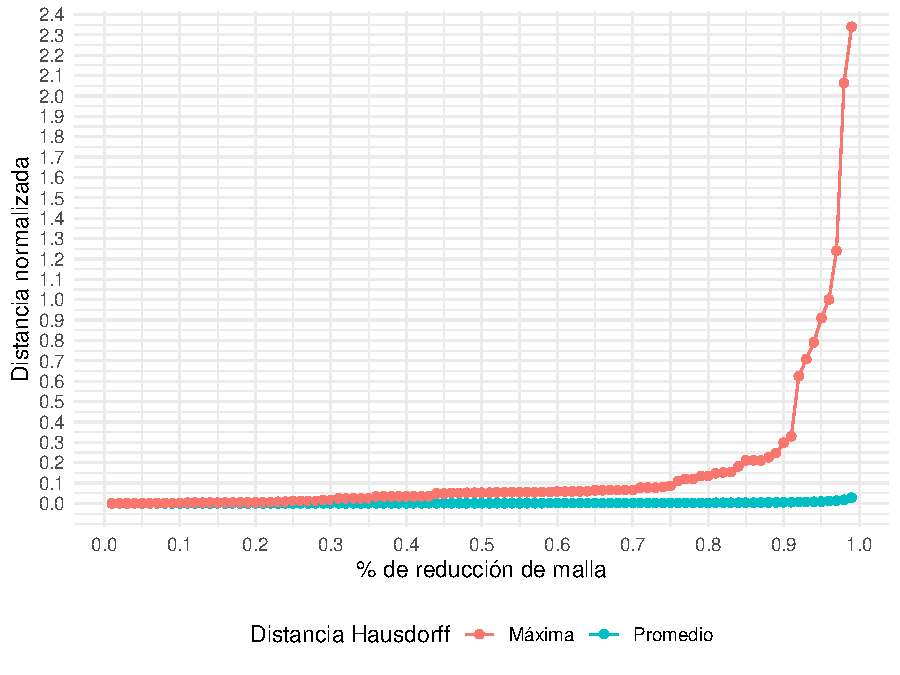
\includegraphics[width=\linewidth]{figures/5_experiments/mesh_redux_study.pdf}
    \caption[Estudio de reducción de mallas]{Distancia Hausdorff normalizada entre las mallas originales y sus versiones reducidas a distintos porcentajes del número original de triángulos. En este experimento, la reducción se realizó en incrementos del 1\%. Se observa que la distancia entre las mallas reducidas y las originales posee valores muy bajos hasta llegar al 90\% de reducción del tamaño original.}
    \label{fig5:redux_study}
\end{figure}

Para abordar esta cuestión, se diseñó un experimento en el que se toma una malla original y se generan versiones reducidas conservando distintas proporciones del número de triángulos originales (por ejemplo, 75\%, 50\%, 25\%, etc.). Posteriormente, estas versiones simplificadas se comparan con la malla original utilizando la distancia de Hausdorff, con el fin de cuantificar la desviación de la superficie resultante respecto de la original.

En la Figura \ref{fig5:redux_study} se presenta la evolución de la distancia Hausdorff normalizada al reducir progresivamente el número de triángulos de las mallas. Esta distancia ha sido normalizada respecto a la diagonal de la \textit{bounding box} de cada malla original, lo que permite comparar directamente las deformaciones relativas entre mallas de diferentes tamaños y complejidades geométricas. Además, esta normalización facilita el cálculo de promedios globales entre las distintas muestras evaluadas.

Como puede observarse, hasta una reducción del 75\% del número de triángulos, el error promedio permanece esencialmente cercano a cero, lo que sugiere una alta fidelidad en la preservación de la geometría original. Durante este mismo rango, el error máximo crece lentamente, manteniéndose al rededor del 0.2\% de variación con respecto a la malla original. Es únicamente a partir de reducciones superiores al 90\% cuando se observa un incremento más pronunciado del error máximo, aunque el error promedio aún se mantiene relativamente controlado.

Estos resultados apuntan a que es posible aplicar reducciones agresivas en la cantidad de triángulos sin comprometer significativamente la calidad topológica de las mallas. En consecuencia, se valida la viabilidad de utilizar versiones simplificadas de las mallas para el entrenamiento por medio de ExMeshCNN.

\subsection{Experimentos con etiqueta única}
Una vez validado que es factible utilizar versiones reducidas de las mallas sin pérdida significativa de información, y habiendo preparado los datos para su uso con el modelo ExMeshCNN, tal como se describe en la Sección \ref{section4:data_preparation}, se procedió a diseñar la estrategia para la generación automática de arquitecturas, explicada en profundidad en la Sección \ref{section4:nas}.

En esta fase, se llevaron a cabo los denominados experimentos de etiqueta única, donde se entrena un modelo independiente para cada una de las características de Todd, sin considerar la influencia de las demás características.

Por cada característica, se realizaron 6 ejecuciones distintas resultantes de las combinaciones de los siguientes parámetros:

\begin{itemize}
\item \textbf{Resolución de la malla}: 100,000 (o 100K); 50,000 (50K) y 25,000 (25K) triángulos.
\item \textbf{Tipo de malla}: Malla completa (Full) o malla recortada (Cut).
\end{itemize}

Cada ejecución implicó la realización de 200 entrenamientos utilizando Optuna para la búsqueda de arquitectura neuronal y optimización de hiperparámetros, con el fin de obtener el modelo más adecuado para predecir cada característica de forma individual.

Dado que se tienen 9 características de Todd, y para cada una se ejecutaron 6 combinaciones con 200 entrenamientos, el número total de entrenamientos realizados asciende a $9\times6\times200=10,800$ entrenamientos totales.

Esto equivale a $1,800$ entrenamientos por característica, lo que refleja el alto grado de exploración llevado a cabo para asegurar un modelo óptimo en cada caso.

\begin{table}[h]
    \centering
    \begin{tabular}{|c|c|c|c|c|}
    \hline
    \rowcolor[HTML]{D33333} 
    {\color[HTML]{FFFFFF} Característica} & {\color[HTML]{FFFFFF} Test Accuracy} & {\color[HTML]{FFFFFF} Test F1} & {\color[HTML]{FFFFFF} Resolución} & {\color[HTML]{FFFFFF} Tipo} \\ \hline
    AF & 0.6546 & 0.4729 & 50K & Cut \\
    BN & 0.9158 & 0.6916 & 25K & Cut \\
    DM & 0.7333 & 0.6261 & 25K & Cut \\
    DP & 0.8827 & 0.7113 & 25K & Cut \\
    IP & 0.7113 & 0.5410 & 100K & Cut \\
    LSE & 0.9800 & 0.9232 & 100K & Full \\
    USE & 0.9797 & 0.8281 & 25K & Cut \\
    VB & 0.5202 & 0.5275 & 50K & Cut \\
    VM & 0.6954 & 0.6747 & 50K & Cut \\ \hline
    \end{tabular}
    \caption{Cuadro resumen de los mejores modelos obtenidos para cada característica}
    \label{table5:single_tag__results}
\end{table}

Como se puede observar en la Tabla \ref{table5:single_tag__results}, existe una considerable variabilidad en los valores obtenidos para la métrica F1 al evaluar cada modelo sobre el conjunto de test. No obstante, en la mayoría de los casos se han alcanzado resultados satisfactorios, con valores de F1 superiores a 0.5 en todos los modelos, además de un \textit{accuracy} generalmente elevado.

Es particularmente destacable el desempeño de las características LSE y USE, que han alcanzado resultados sobresalientes a pesar de presentar un alto grado de desbalance en las etiquetas, como se evidenció en el EDA (Sección \ref{section4:data_eda}). Esto sugiere la presencia de patrones bien definidos en la superficie ósea que han sido correctamente capturados por los modelos, permitiendo lograr simultáneamente un \textit{accuracy} muy alto y valores de F1 igualmente notables. En contraste, otras dos características también altamente desbalanceadas, como BN y DP, si bien obtuvieron buenos resultados, se encuentran dentro del rango de desempeño general de las demás características más balanceadas, lo que refuerza la hipótesis de que LSE y USE presentan una topología más informativa o distinguible para las redes.

Por otro lado, la característica VB, que presenta la distribución más balanceada de etiquetas, fue la que obtuvo el rendimiento más bajo tanto en términos de \textit{accuracy} como de F1. Esto podría indicar que, pese a un buen balance, los patrones topológicos asociados a esta característica son más sutiles o complejos de identificar, lo cual plantea un reto adicional para el modelo.

El resto de las características muestran un comportamiento relativamente uniforme, sin una clara correlación entre el grado de desbalance y el rendimiento del modelo, lo que a su vez sugiere que el enfoque de entrenamiento adoptado ha sido eficaz para extraer información relevante incluso en escenarios con clases altamente desbalanceadas y una cantidad limitada de datos.

Un aspecto adicional a destacar es el impacto del tipo de malla utilizada. Exceptuando el modelo de LSE, todos los demás alcanzaron mejores resultados al emplear las versiones recortadas de las mallas. Este comportamiento respalda la hipótesis de que eliminar estructuras óseas irrelevantes (según la práctica de los expertos) permite concentrar el poder de representación del modelo en la zona de interés, reduciendo el ruido y facilitando la identificación de patrones significativos. En el caso de LSE, sin embargo, las mallas completas resultaron más beneficiosas, lo cual podría implicar que la información relevante para esta característica se encuentra distribuida también fuera de la región habitualmente considerada como de interés.

Respecto a la resolución, se observa que los mejores resultados, en general, se obtuvieron con la resolución más baja de 25K triángulos, seguida de 50K, y solo dos modelos alcanzaron su mejor desempeño con 100K triángulos. Esta observación concuerda con lo reportado por los autores de ExMeshCNN \cite{kim_exmeshcnn_2022}, donde también se encontró que las mallas de menor resolución producían mejores resultados. Se teoriza que esto se debe a que, al aumentar la resolución, la operación de \textit{global average pooling} que conecta las capas convolucionales con las totalmente conectadas podría estar diluyendo información crítica al comprimir un mayor número de triángulos en una única representación.

Sin embargo, las características LSE e IP constituyen una excepción a esta tendencia: en ambos casos, la mayor resolución permitió obtener un mejor rendimiento, lo que indica que para estas características el mayor nivel de detalle en la superficie ósea proporciona una ventaja en el aprendizaje del modelo.

\subsection{Experimentos multietiqueta}
Una vez realizados los experimentos de etiqueta única, se procedió a entrenar modelos capaces de predecir múltiples características simultáneamente. Para ello, se empleó el enfoque de \textit{multi-label classification}, que permite que cada muestra del conjunto de datos pueda estar asociada a más de una etiqueta, en contraste con la clasificación tradicional donde cada muestra pertenece a una única clase.

Para estos experimentos, primero se realizaron ejecuciones con todas las características de Todd por cada resolución, tipo de malla y, adicionalmente, dos configuraciones de la parte densa o totalmente conectada del modelo: una donde todas las salidas poseen la misma estructura y otra donde cada salida tiene una estructura densa independiente.

Posteriormente se realizaron experimentos con la mejor configuración obtenida en los resultados de etiqueta única para cada característica y las 3 características que presentan mayor correlación a la misma, como se puede observar en la Tabla \ref{table4:corr}, variando las dos configuraciones de la parte densa de la red.

Se realizaron $2 \times 2 \times 3 \times 200 = 2,400$ experimentos con todas las características, $9 \times 2 \times 200 = 3,600$ experimentos con las top 3 características con mayor asociación a una característica dada. De estos 6000 entrenamientos, en la Tabla \ref{table5:multilabel_results} se muestran los resultados de los mejores modelos obtenidos para cada característica.

\begin{table}[h]
    \centering
    \resizebox{\textwidth}{!}{%
    \begin{tabular}{|cc|c|c|c|c|c|}
        \hline
        \rowcolor[HTML]{D33333} 
        \multicolumn{2}{|c|}{\cellcolor[HTML]{D33333}{\color[HTML]{FFFFFF} \textbf{Característica}}} & \cellcolor[HTML]{D33333}{\color[HTML]{FFFFFF} } & \cellcolor[HTML]{D33333}{\color[HTML]{FFFFFF} } & \cellcolor[HTML]{D33333}{\color[HTML]{FFFFFF} } & \cellcolor[HTML]{D33333}{\color[HTML]{FFFFFF} } & \cellcolor[HTML]{D33333}{\color[HTML]{FFFFFF} } \\ \cline{1-2}
        \rowcolor[HTML]{D33333} 
        \multicolumn{1}{|c|}{\cellcolor[HTML]{D33333}{\color[HTML]{FFFFFF} \textbf{Evaluada}}} & {\color[HTML]{FFFFFF} \textbf{Soporte}} & \multirow{-2}{*}{\cellcolor[HTML]{D33333}{\color[HTML]{FFFFFF} \textbf{\begin{tabular}[c]{@{}c@{}}Test \\ Acc\end{tabular}}}} & \multirow{-2}{*}{\cellcolor[HTML]{D33333}{\color[HTML]{FFFFFF} \textbf{\begin{tabular}[c]{@{}c@{}}Test \\ F1\end{tabular}}}} & \multirow{-2}{*}{\cellcolor[HTML]{D33333}{\color[HTML]{FFFFFF} \textbf{Resolución}}} & \multirow{-2}{*}{\cellcolor[HTML]{D33333}{\color[HTML]{FFFFFF} \textbf{Hueso}}} & \multirow{-2}{*}{\cellcolor[HTML]{D33333}{\color[HTML]{FFFFFF} \textbf{Estructura Densa}}} \\ \hline
        \multicolumn{1}{|c|}{AF} & DM, LSE, USE & 0.6888 & 0.5164 & 50K & Cut & Variable \\
        \multicolumn{1}{|c|}{BN} & AF, DP, LSE & 0.9141 & 0.7869 & 25K & Cut & Variable \\
        \multicolumn{1}{|c|}{DM} & Todas & 0.7980 & 0.6525 & 100K & Cut & Same \\
        \multicolumn{1}{|c|}{DP} & Todas & 0.9261 & 0.7215 & 100K & Cut & Same \\
        \multicolumn{1}{|c|}{IP} & Todas & 0.6749 & 0.4777 & 50K & Full & Same \\
        \multicolumn{1}{|c|}{LSE} & DM, USE, VM & 0.9495 & 0.7942 & 100K & Full & Variable \\
        \multicolumn{1}{|c|}{USE} & AF, DM, LSE & 0.9541 & 0.8588 & 25K & Cut & Same \\
        \multicolumn{1}{|c|}{VB} & Todas & 0.4926 & 0.4775 & 50K & Cut & Same \\
        \multicolumn{1}{|c|}{VM} & AF, DM, IP & 0.6954 & 0.4975 & 100K & Cut & Variable \\ \hline
    \end{tabular}%
    }
    \caption{Resultados de los mejores modelos obtenidos para cada característica en los experimentos multietiqueta.}
    \label{table5:multilabel_results}
    \end{table}

De los resultados obtenidos, se observa que existe más variedad respecto a la resolución de las mallas empleadas. Sorpresivamente, se encuentran casi de forma equitativa las resoluciones de 25K, 50K y 100K triángulos, con 4 modelos utilizando 100K, 3 modelos con 50K y 2 modelos con 25K. Esto contrasta con los experimentos de etiqueta única, donde la mayoría de los modelos se entrenaron con mallas de 25K triángulos. Esto resulta interesante porque sugiere que, al entrenar modelos multietiqueta, la información contenida en las mallas de mayor resolución puede ser más relevante para la predicción de múltiples características simultáneamente.

Por parte de los tipos de malla, esto se ha mantenido constante respecto a los experimentos de etiqueta única, ya que la mayoría de los modelos se entrenaron con mallas recortadas (Cut), excepto en el caso de las características LSE e IP, que emplearon mallas completas (Full). Esto refuerza la idea de que, para ciertas características, la información contenida en las zonas no recortadas es crucial para lograr un buen rendimiento del modelo incluso en un contexto multietiqueta.

En cuanto a la estructura de las capas totalmente conectadas, se observa que no hay una preferencia clara entre las distintas configuraciones, estando distribuidas casi equitativamente, esto sugiere que la elección de la estructura densa puede depender más de la naturaleza específica de las características a predecir que de una tendencia generalizada.

Sobre las características de soporte, nuevamente se encuentra una distribución casi equitativa entre hacer uso de todas las características o las tres más correlacionadas con la característica a predecir. Esto indica que, al entrenar modelos multietiqueta, es beneficioso considerar un conjunto amplio de características para mejorar la capacidad predictiva del modelo, no existiendo una tendencia clara hacia un enfoque u otro, al menos en estos experimentos.

\begin{table}[h]
    \centering
    \begin{tabular}{|c|cc|cc|}
        \hline
        \rowcolor[HTML]{D33333} 
        \cellcolor[HTML]{D33333}{\color[HTML]{FFFFFF} } & \multicolumn{2}{c|}{\cellcolor[HTML]{D33333}{\color[HTML]{FFFFFF} \textbf{Etiqueta Única}}} & \multicolumn{2}{c|}{\cellcolor[HTML]{D33333}{\color[HTML]{FFFFFF} \textbf{Etiqueta Múltiple}}} \\ \cline{2-5} 
        \rowcolor[HTML]{D33333} 
        \multirow{-2}{*}{\cellcolor[HTML]{D33333}{\color[HTML]{FFFFFF} \textbf{Característica}}} & \multicolumn{1}{c|}{\cellcolor[HTML]{D33333}{\color[HTML]{FFFFFF} \textbf{Test Acc}}} & {\color[HTML]{FFFFFF} \textbf{Test F1}} & \multicolumn{1}{c|}{\cellcolor[HTML]{D33333}{\color[HTML]{FFFFFF} \textbf{Test Acc}}} & {\color[HTML]{FFFFFF} \textbf{Test F1}} \\ \hline
        AF & \multicolumn{1}{c|}{0.6546} & 0.4729 & \multicolumn{1}{c|}{0.6888} & \textbf{0.5164} \\
        BN & \multicolumn{1}{c|}{0.9158} & 0.6916 & \multicolumn{1}{c|}{0.9141} & \textbf{0.7869} \\
        DM & \multicolumn{1}{c|}{0.7333} & 0.6261 & \multicolumn{1}{c|}{0.7980} & \textbf{0.6525} \\
        DP & \multicolumn{1}{c|}{0.8827} & 0.7113 & \multicolumn{1}{c|}{0.9261} & \textbf{0.7215} \\
        IP & \multicolumn{1}{c|}{0.7113} & \textbf{0.541} & \multicolumn{1}{c|}{0.6749} & 0.4777 \\
        LSE & \multicolumn{1}{c|}{0.9800} & \textbf{0.9232} & \multicolumn{1}{c|}{0.9495} & 0.7942 \\
        USE & \multicolumn{1}{c|}{0.9797} & 0.8281 & \multicolumn{1}{c|}{0.9541} & \textbf{0.8588} \\
        VB & \multicolumn{1}{c|}{0.5202} & \textbf{0.5275} & \multicolumn{1}{c|}{0.4926} & 0.4775 \\
        VM & \multicolumn{1}{c|}{0.6954} & \textbf{0.6747} & \multicolumn{1}{c|}{0.6954} & 0.4975 \\ \hline
    \end{tabular}
    \caption[Comparación de resultados entre los mejores modelos obtenidos en los experimentos de etiqueta única y multietiqueta]{Comparación de resultados entre los mejores modelos obtenidos en los experimentos de etiqueta única y multietiqueta. Los valores en negrita indican los mejores resultados obtenidos de la métrica F1 para cada característica.}
    \label{table5:multilabel_comparison}
\end{table}

Finalmente, se observa que los resultados obtenidos en los experimentos multietiqueta son en general superiores a los de etiqueta única, observándose la Tabla \ref{table5:multilabel_comparison}, dónde 6 de las 9 características mejoran la métrica F1 respecto a sus contrapartes de etiqueta única. Esto sugiere que el modelo es capaz de aprender patrones más complejos y representativos al considerar múltiples características simultáneamente, lo que a su vez puede mejorar la generalización del modelo y su capacidad para capturar relaciones entre las distintas características. Siendo esto consistente con la literatura consultada, donde se ha demostrado que los modelos multietiqueta pueden beneficiarse de la correlación entre las etiquetas para mejorar el rendimiento general del modelo \cite{ranjan_hyperface_2019}.

Si bien existe más disparidad respecto al \textit{accuracy} entre los experimentos de etiqueta única y multietiqueta, en general se observa que se mantiene un rendimiento alto en ambas configuraciones, con valores muy similares a los obtenidos en los experimentos de etiqueta única.

\section{Análisis de Resultados}

Durante los experimentos realizados, se ha observado que el modelo ExMeshCNN es capaz de aprender patrones topológicos relevantes en las mallas óseas para predecir las características de Todd. Los resultados obtenidos tanto en los experimentos de etiqueta única como en los de multietiqueta muestran un rendimiento prometedor, con valores de F1 y \textit{accuracy} que evidencian una buena capacidad de generalización por parte de los modelos, optimizados mediante búsqueda automática de arquitectura e hiperparámetros.

Al analizar las matrices de confusión de los mejores modelos (Figuras \ref{fig5:AF_confusion_matrix}, \ref{fig5:BN_confusion_matrix}, \ref{fig5:DM_confusion_matrix}, \ref{fig5:DP_confusion_matrix}, \ref{fig5:IP_confusion_matrix}, \ref{fig5:LSE_confusion_matrix}, \ref{fig5:USE_confusion_matrix}, \ref{fig5:VB_confusion_matrix} y \ref{fig5:VM_confusion_matrix}), se aprecia que los modelos tienden a clasificar correctamente la mayoría de las muestras de una forma equilibrada tal y como se observó con la métrica F1, cometiendo más errores en aquellas clases menos representadas. Este comportamiento es coherente con lo esperado en problemas de clasificación desbalanceada, donde los modelos suelen favorecer las clases mayoritarias. No obstante, la mayoría de las confusiones ocurren entre clases adyacentes, lo que sugiere que el modelo ha aprendido a distinguir de manera significativa los patrones de las distintas características de Todd. De forma particular, la característica con peor rendimiento es VB, que presenta una matriz de confusión con un alto número de falsos negativos, lo que indica que el modelo tiene dificultades para identificar correctamente las muestras de esta clase, a pesar de que es la característica más balanceada en términos de distribución de etiquetas. Esto concuerda con las observaciones realizadas en en ???, dónde se observó que esta característica es la que presenta la mayor tasa de error inter e intra-experto, lo que sugiere que esta es una característica más subjetiva o menos consistente entre los expertos, lo que dificulta su clasificación por parte del modelo.

\subsection{Hiperparámetros y Arquitectura Neuronal}
Para facilitar la comprensión, se incluye una tabla resumen que detalla los datos de entrada utilizados por cada modelo, así como su arquitectura y los hiperparámetros seleccionados. La Tabla \ref{table5:sample_table} muestra un ejemplo del formato empleado, junto con la explicación de cada una de sus columnas y filas.

Los mejores modelos obtenidos presentan configuraciones arquitectónicas notablemente diversas entre sí, lo que indica que la búsqueda automática ha sido efectiva para adaptar la estructura de las redes a los requerimientos específicos de cada característica.

Pese a esta diversidad, se observa una tendencia general hacia redes con mayor profundidad en las capas convolucionales, como en los casos de AF (Tabla \ref{table5:AF_best_model}), BN (Tabla \ref{table5:BN_best_model}), IP (Tabla \ref{table5:IP_best_model}), LSE (Tabla \ref{table5:LSE_best_model}), VB (Tabla \ref{table5:VB_best_model}) y VM (Tabla \ref{table5:VM_best_model}), donde se utilizaron 4 o más capas convolucionales, y algunas, como AF, BN y VM, alcanzaron hasta 6 capas. Esto sugiere que estas características pueden requerir una mayor capacidad de representación para capturar los patrones complejos presentes en las mallas.

En cuanto al número de filtros por capa, se aprecia un patrón común de expansión y contracción a lo largo de la red, posiblemente reflejando una estructura tipo cuello de botella. USE (Tabla \ref{table5:USE_best_model}) es la única excepción donde este patrón no se manifiesta claramente.

Las capas totalmente conectadas, en cambio, presentan mayor variabilidad en cuanto al número de neuronas y estructura, sin un patrón claro, lo que indica una fuerte dependencia del diseño respecto a la tarea específica.

En términos de hiperparámetros, se detecta un uso consistente del optimizador Adam y de la inicialización Kaiming en la mayoría de los modelos exitosos, lo que sugiere que estas configuraciones son adecuadas para el entrenamiento de redes basadas en ExMeshCNN. En cuanto a las funciones de pérdida, predomina el uso de WCE, seguida por CBL, lo cual es coherente con la naturaleza desbalanceada del problema y valida su idoneidad para este tipo de clasificación.

\begin{figure}[p]
    \begin{minipage}{\linewidth}
        \centering
        \begin{tabular}{c|cc|c|c|}
            \hline
            \rowcolor[HTML]{D33333} 
            \multicolumn{1}{|c|}{\cellcolor[HTML]{D33333}{\color[HTML]{FFFFFF} }} & \multicolumn{2}{c|}{\cellcolor[HTML]{D33333}{\color[HTML]{FFFFFF} \textbf{DECR}}} & {\color[HTML]{FFFFFF} \textbf{CONV}} & {\color[HTML]{FFFFFF} \textbf{FN}} \\ \cline{2-5} 
            \multicolumn{1}{|c|}{\multirow{-2}{*}{\cellcolor[HTML]{D33333}{\color[HTML]{FFFFFF} \textbf{DATA}}}} & \multicolumn{2}{c|}{\cellcolor[HTML]{D33333}{\color[HTML]{FFFFFF} \textbf{GEOD}}} &  & \textbf{(h)} \\ \cline{1-3} \cline{5-5} 
            \multicolumn{1}{|c|}{\cellcolor[HTML]{D33333}{\color[HTML]{FFFFFF} \textbf{RES}}} & MID & (c) &  &  \\ \cline{1-1}
            \multicolumn{1}{|c|}{(a)} & OUT & (d) &  &  \\ \cline{1-3}
            \multicolumn{1}{|c|}{\cellcolor[HTML]{D33333}{\color[HTML]{FFFFFF} \textbf{TYPE}}} & \multicolumn{2}{c|}{\cellcolor[HTML]{D33333}{\color[HTML]{FFFFFF} \textbf{GEOM}}} &  &  \\ \cline{1-3}
            \multicolumn{1}{|c|}{(b)} & MID & (e) &  &  \\ \cline{1-1}
             & OUT & (f) & \multirow{-6}{*}{(g)} & \multirow{-5}{*}{(i)} \\ \cline{2-5} 
        \end{tabular}
    
        \vspace{1em}
    
        \begin{tabular}{|
            >{\columncolor[HTML]{D33333}}c |c|c|}
            \hline
            {\color[HTML]{FFFFFF} \textbf{LR}} & (j) & \cellcolor[HTML]{D33333}{\color[HTML]{FFFFFF} \textbf{LOSS}} \\ \hline
            {\color[HTML]{FFFFFF} \textbf{OPTIMIZER}} & (k) & \textbf{(h)} \\ \hline
            {\color[HTML]{FFFFFF} \textbf{INIT}} & (l) & (n) \\ \hline
        \end{tabular}
        \captionof{table}[Formato de tabla usado para resumir los datos de entrada, la estructura de la red y los hiperparámetros de los mejores modelos]{Formato utilizado para resumir los datos de entrada, la estructura de la red y los hiperparámetros empleados en cada uno de los modelos. La tabla superior detalla las configuraciones relativas a los datos y la arquitectura, mientras que la tabla inferior resume los hiperparámetros principales. En la tabla superior, la columna \textbf{DATA} especifica las características de los datos de entrada: \textbf{RES} indica la resolución de la malla (a) y \textbf{TYPE} su tipo (b). La columna \textbf{DECR} incluye la configuración de los descriptores utilizados: \textbf{GEOD} para el descriptor geodésico y \textbf{GEOM} para el descriptor geométrico; MID y OUT indican respectivamente la densidad de sus capas intermedias (c, e) y de salida (d, f). La columna \textbf{CONV} muestra la arquitectura de las capas convolucionales: número de capas y densidad de cada una (g). La columna \textbf{FN} presenta en (h) las características morfológicas predichas y en (i) la configuración de la parte densa del modelo de cada una. En la tabla inferior, \textbf{LR} indica la tasa de aprendizaje (j), \textbf{OPTIMIZER} el optimizador empleado (k), \textbf{INIT} el tipo de inicialización de pesos (l), y \textbf{LOSS} la función de pérdida (n) asociada a la característica correspondiente (h).}
        \label{table5:sample_table}
    \end{minipage}
\end{figure}

%% AF
\begin{figure}[htbp]
    \centering
    % --- Top: Table ---
    \begin{minipage}{\linewidth}
        \centering
        \begin{tabular}{c|cc|c|cccc|}
            \hline
            \rowcolor[HTML]{D33333} 
            \multicolumn{1}{|c|}{\cellcolor[HTML]{D33333}{\color[HTML]{FFFFFF} }} & \multicolumn{2}{c|}{\cellcolor[HTML]{D33333}{\color[HTML]{FFFFFF} \textbf{DECR}}} & {\color[HTML]{FFFFFF} \textbf{CONV}} & \multicolumn{4}{c|}{\cellcolor[HTML]{D33333}{\color[HTML]{FFFFFF} \textbf{FN}}} \\ \cline{2-8} 
            \multicolumn{1}{|c|}{\multirow{-2}{*}{\cellcolor[HTML]{D33333}{\color[HTML]{FFFFFF} \textbf{DATA}}}} & \multicolumn{2}{c|}{\cellcolor[HTML]{D33333}{\color[HTML]{FFFFFF} \textbf{GEOD}}} & 64 & \multicolumn{1}{c|}{\cellcolor[HTML]{FFCCC9}\textbf{AF}} & \multicolumn{1}{c|}{\cellcolor[HTML]{FFFFFF}\textbf{DM}} & \multicolumn{1}{c|}{\textbf{LSE}} & \textbf{USE} \\ \cline{1-3} \cline{5-8} 
            \multicolumn{1}{|c|}{\cellcolor[HTML]{D33333}{\color[HTML]{FFFFFF} \textbf{RES}}} & MID & 16 & 32 & \multicolumn{1}{c|}{\cellcolor[HTML]{FFCCC9}256} & \multicolumn{1}{c|}{\cellcolor[HTML]{FFFFFF}8} & \multicolumn{1}{c|}{16} & 32 \\ \cline{1-1} \cline{5-6}
            \multicolumn{1}{|c|}{50K} & OUT & 128 & 32 &  & \multicolumn{1}{c|}{\cellcolor[HTML]{FFFFFF}} & \multicolumn{1}{c|}{8} & 32 \\ \cline{1-3}
            \multicolumn{1}{|c|}{\cellcolor[HTML]{D33333}{\color[HTML]{FFFFFF} \textbf{TYPE}}} & \multicolumn{2}{c|}{\cellcolor[HTML]{D33333}{\color[HTML]{FFFFFF} \textbf{GEOM}}} & 128 &  & \multicolumn{1}{c|}{} & \multicolumn{1}{c|}{64} & 256 \\ \cline{1-3}
            \multicolumn{1}{|c|}{Cut} & MID & 128 & 256 &  & \multicolumn{1}{c|}{} & \multicolumn{1}{c|}{128} & 64 \\ \cline{1-1} \cline{7-7}
             & OUT & 256 & 32 &  &  & \multicolumn{1}{c|}{} & 16 \\ \cline{2-4} \cline{8-8} 
        \end{tabular}

        \vspace{1em}

        \begin{tabular}{|
            >{\columncolor[HTML]{D33333}}c |c|
            >{\columncolor[HTML]{FFCCC9}}c ccc|}
            \hline
            {\color[HTML]{FFFFFF} \textbf{LR}} & $3.4261 \times 10^{-4}$ & \multicolumn{4}{c|}{\cellcolor[HTML]{D33333}{\color[HTML]{FFFFFF} \textbf{LOSS}}} \\ \hline
            {\color[HTML]{FFFFFF} \textbf{OPTIMIZER}} & AdamW & \multicolumn{1}{c|}{\cellcolor[HTML]{FFCCC9}\textbf{AF}} & \multicolumn{1}{c|}{\textbf{DM}} & \multicolumn{1}{c|}{\textbf{LSE}} & \textbf{USE} \\ \hline
            {\color[HTML]{FFFFFF} \textbf{INIT}} & N/A & \multicolumn{1}{c|}{\cellcolor[HTML]{FFCCC9}WCE} & \multicolumn{1}{c|}{WCE} & \multicolumn{1}{c|}{CE} & WCE \\ \hline
        \end{tabular}
        \captionof{table}{Característica AF: Datos de entrada, estructura de red e hiperparámetros del mejor modelo.}
        \label{table5:AF_best_model}
    \end{minipage}

    \vspace{1.5em} % vertical space between table and image

    % --- Bottom: Figure ---
    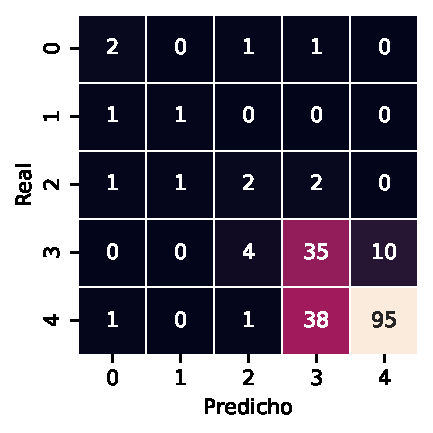
\includegraphics[width=0.6\linewidth]{figures/5_experiments/multi-af-cm.pdf}
    \caption[Característica AF: Matriz de confusión del mejor modelo en datos de test]{Característica \textbf{AF}: Matriz de confusión del mejor modelo en datos de test. Leyenda: \textbf{0}: Porosidad Regular, \textbf{1}: Muy Definidas, \textbf{2}: Poco Profundas, \textbf{3}: Restos de Surcos, \textbf{4}: No hay surcos.}
    \label{fig5:AF_confusion_matrix}
\end{figure}

%% BN
\begin{figure}[htbp]
    \centering
    % --- Top: Table ---
    \begin{minipage}{\linewidth}
        \centering
        \begin{tabular}{c|cc|c|cccc}
            \hline
            \rowcolor[HTML]{D33333} 
            \multicolumn{1}{|c|}{\cellcolor[HTML]{D33333}{\color[HTML]{FFFFFF} }} & \multicolumn{2}{c|}{\cellcolor[HTML]{D33333}{\color[HTML]{FFFFFF} \textbf{DECR}}} & {\color[HTML]{FFFFFF} \textbf{CONV}} & \multicolumn{4}{c|}{\cellcolor[HTML]{D33333}{\color[HTML]{FFFFFF} \textbf{FN}}} \\ \cline{2-8} 
            \multicolumn{1}{|c|}{\multirow{-2}{*}{\cellcolor[HTML]{D33333}{\color[HTML]{FFFFFF} \textbf{DATA}}}} & \multicolumn{2}{c|}{\cellcolor[HTML]{D33333}{\color[HTML]{FFFFFF} \textbf{GEOD}}} & 256 & \multicolumn{1}{c|}{\cellcolor[HTML]{FFFFFF}\textbf{AF}} & \multicolumn{1}{c|}{\cellcolor[HTML]{FFCCC9}\textbf{BN}} & \multicolumn{1}{c|}{\textbf{DP}} & \multicolumn{1}{c|}{\textbf{LSE}} \\ \cline{1-3} \cline{5-8} 
            \multicolumn{1}{|c|}{\cellcolor[HTML]{D33333}{\color[HTML]{FFFFFF} \textbf{RES}}} & MID & 256 & 128 & \multicolumn{1}{c|}{\cellcolor[HTML]{FFFFFF}128} & \multicolumn{1}{c|}{\cellcolor[HTML]{FFCCC9}32} & \multicolumn{1}{c|}{32} & \multicolumn{1}{c|}{32} \\ \cline{1-1} \cline{5-5}
            \multicolumn{1}{|c|}{25K} & OUT & 16 & 256 & \multicolumn{1}{c|}{} & \multicolumn{1}{c|}{\cellcolor[HTML]{FFCCC9}64} & \multicolumn{1}{c|}{64} & \multicolumn{1}{c|}{128} \\ \cline{1-3} \cline{6-6}
            \multicolumn{1}{|c|}{\cellcolor[HTML]{D33333}{\color[HTML]{FFFFFF} \textbf{TYPE}}} & \multicolumn{2}{c|}{\cellcolor[HTML]{D33333}{\color[HTML]{FFFFFF} \textbf{GEOM}}} & 64 &  & \multicolumn{1}{c|}{} & \multicolumn{1}{c|}{256} & \multicolumn{1}{c|}{128} \\ \cline{1-3} \cline{8-8} 
            \multicolumn{1}{|c|}{Cut} & MID & 32 & 16 &  & \multicolumn{1}{c|}{} & \multicolumn{1}{c|}{16} &  \\ \cline{1-1}
             & OUT & 16 & 64 &  & \multicolumn{1}{c|}{} & \multicolumn{1}{c|}{256} &  \\ \cline{2-4} \cline{7-7}
        \end{tabular}

        \vspace{1em}

        \begin{tabular}{|
            >{\columncolor[HTML]{D33333}}c |c|c
            >{\columncolor[HTML]{FFCCC9}}c cc|}
            \hline
            {\color[HTML]{FFFFFF} \textbf{LR}} & $5.0965 \times 10^{-3}$ & \multicolumn{4}{c|}{\cellcolor[HTML]{D33333}{\color[HTML]{FFFFFF} \textbf{LOSS}}} \\ \hline
            {\color[HTML]{FFFFFF} \textbf{OPTIMIZER}} & Radam & \multicolumn{1}{c|}{\textbf{AF}} & \multicolumn{1}{c|}{\cellcolor[HTML]{FFCCC9}\textbf{BN}} & \multicolumn{1}{c|}{\textbf{DP}} & \textbf{LSE} \\ \hline
            {\color[HTML]{FFFFFF} \textbf{INIT}} & Kaiming & \multicolumn{1}{c|}{FL} & \multicolumn{1}{c|}{\cellcolor[HTML]{FFCCC9}CBL} & \multicolumn{1}{c|}{CBL} & CBL \\ \hline
        \end{tabular}
        \captionof{table}{Característica BN: Datos de entrada, estructura de red e hiperparámetros del mejor modelo.}
        \label{table5:BN_best_model}
    \end{minipage}

    \vspace{1.5em} % vertical space between table and image

    % --- Bottom: Figure ---
    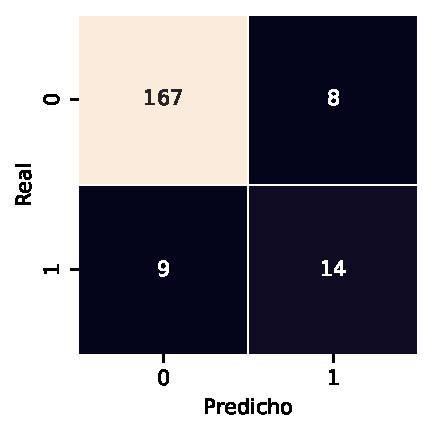
\includegraphics[width=0.6\linewidth]{figures/5_experiments/multi-bn-cm.pdf}
    \caption[Característica BN: Matriz de confusión del mejor modelo en datos de test.]{Característica BN: Matriz de confusión del mejor modelo en datos de test. Leyenda: \textbf{0}: Ausente, \textbf{1}: Presente.}
    \label{fig5:BN_confusion_matrix}
\end{figure}

%% DM / DP
\begin{figure}[htbp]
    \centering
    % --- Top: Table ---
    \begin{minipage}{\linewidth}
        \centering
        \begin{tabular}{c|cc|cc}
            \hline
            \rowcolor[HTML]{D33333} 
            \multicolumn{1}{|c|}{\cellcolor[HTML]{D33333}{\color[HTML]{FFFFFF} }} & \multicolumn{2}{c|}{\cellcolor[HTML]{D33333}{\color[HTML]{FFFFFF} \textbf{DECR}}} & \multicolumn{1}{c|}{\cellcolor[HTML]{D33333}{\color[HTML]{FFFFFF} \textbf{CONV}}} & \multicolumn{1}{c|}{\cellcolor[HTML]{D33333}{\color[HTML]{FFFFFF} \textbf{FN}}} \\ \cline{2-5} 
            \multicolumn{1}{|c|}{\multirow{-2}{*}{\cellcolor[HTML]{D33333}{\color[HTML]{FFFFFF} \textbf{DATA}}}} & \multicolumn{2}{c|}{\cellcolor[HTML]{D33333}{\color[HTML]{FFFFFF} \textbf{GEOD}}} & \multicolumn{1}{c|}{64} & \multicolumn{1}{c|}{\textbf{Todos}} \\ \cline{1-3} \cline{5-5} 
            \multicolumn{1}{|c|}{\cellcolor[HTML]{D33333}{\color[HTML]{FFFFFF} \textbf{RES}}} & MID & 16 & \multicolumn{1}{c|}{128} & \multicolumn{1}{c|}{32} \\ \cline{1-1} \cline{5-5} 
            \multicolumn{1}{|c|}{100K} & OUT & 16 & \multicolumn{1}{c|}{128} &  \\ \cline{1-4}
            \multicolumn{1}{|c|}{\cellcolor[HTML]{D33333}{\color[HTML]{FFFFFF} \textbf{TYPE}}} & \multicolumn{2}{c|}{\cellcolor[HTML]{D33333}{\color[HTML]{FFFFFF} \textbf{GEOM}}} &  &  \\ \cline{1-3}
            \multicolumn{1}{|c|}{Cut} & MID & 16 &  &  \\ \cline{1-1}
             & OUT & 256 &  &  \\ \cline{2-3}
        \end{tabular}

        \vspace{1em}

        \begin{tabular}{cc|ccccc}
        \hline
        \multicolumn{1}{|c|}{\cellcolor[HTML]{D33333}{\color[HTML]{FFFFFF} \textbf{LR}}} & $1.4861 \times 10^{-4}$ & \multicolumn{5}{c|}{\cellcolor[HTML]{D33333}{\color[HTML]{FFFFFF} \textbf{LOSS}}} \\ \hline
        \multicolumn{1}{|c|}{\cellcolor[HTML]{D33333}{\color[HTML]{FFFFFF} \textbf{OPTIMIZER}}} & Adam & \multicolumn{1}{c|}{\textbf{AF}} & \multicolumn{1}{c|}{\textbf{BN}} & \multicolumn{1}{c|}{\cellcolor[HTML]{FFCCC9}\textbf{DM}} & \multicolumn{1}{c|}{\cellcolor[HTML]{FFCCC9}\textbf{DP}} & \multicolumn{1}{c|}{\textbf{IP}} \\ \hline
        \multicolumn{1}{|c|}{\cellcolor[HTML]{D33333}{\color[HTML]{FFFFFF} \textbf{INIT}}} & Kaiming & \multicolumn{1}{c|}{WCE} & \multicolumn{1}{c|}{CE} & \multicolumn{1}{c|}{\cellcolor[HTML]{FFCCC9}CE} & \multicolumn{1}{c|}{\cellcolor[HTML]{FFCCC9}CE} & \multicolumn{1}{c|}{WCE} \\ \hline
        &  & \multicolumn{1}{c|}{\textbf{LSE}} & \multicolumn{1}{c|}{\textbf{USE}} & \multicolumn{1}{c|}{\textbf{VB}} & \multicolumn{1}{c|}{\textbf{VM}} &  \\ \cline{3-6}
        &  & \multicolumn{1}{c|}{CE} & \multicolumn{1}{c|}{WCE} & \multicolumn{1}{c|}{CE} & \multicolumn{1}{c|}{CE} &  \\ \cline{3-6}
        \end{tabular}
        \captionof{table}{Características DP y DM: Datos de entrada, estructura de red e hiperparámetros del mejor modelo.}
        \label{table5:DM_DP_best_model}
    \end{minipage}

    \vspace{1.5em} % vertical space between table and image

    % --- Bottom: Figure ---
    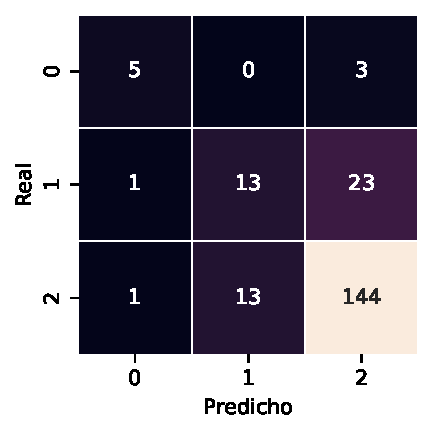
\includegraphics[width=0.4\linewidth]{figures/5_experiments/multi-dm-cm.pdf}
    \caption[Característica DM: Matriz de confusión del mejor modelo en datos de test.]{Característica \textbf{DM}: Matriz de confusión del mejor modelo en datos de test. Leyenda: \textbf{0}: No Definido, \textbf{1}: En Formación, \textbf{2}: Definido.}
    \label{fig5:DM_confusion_matrix}
    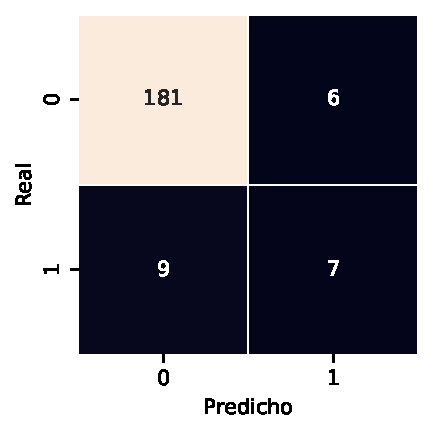
\includegraphics[width=0.4\linewidth]{figures/5_experiments/multi-dp-cm.pdf}
    \caption[Característica DP: Matriz de confusión del mejor modelo en datos de test.]{Característica DP: Matriz de confusión del mejor modelo en datos de test. Leyenda: \textbf{0}: Ausente, \textbf{1}: Presente.}
    \label{fig5:DP_confusion_matrix}
\end{figure}

%% IP
\begin{figure}[htbp]
    \centering
    % --- Top: Table ---
    \begin{minipage}{\linewidth}
        \centering
        \begin{tabular}{c|cc|cc}
            \hline
            \rowcolor[HTML]{D33333} 
            \multicolumn{1}{|c|}{\cellcolor[HTML]{D33333}{\color[HTML]{FFFFFF} }} & \multicolumn{2}{c|}{\cellcolor[HTML]{D33333}{\color[HTML]{FFFFFF} \textbf{DECR}}} & \multicolumn{1}{c|}{\cellcolor[HTML]{D33333}{\color[HTML]{FFFFFF} \textbf{CONV}}} & \multicolumn{1}{c|}{\cellcolor[HTML]{D33333}{\color[HTML]{FFFFFF} \textbf{FN}}} \\ \cline{2-5} 
            \multicolumn{1}{|c|}{\multirow{-2}{*}{\cellcolor[HTML]{D33333}{\color[HTML]{FFFFFF} \textbf{DATA}}}} & \multicolumn{2}{c|}{\cellcolor[HTML]{D33333}{\color[HTML]{FFFFFF} \textbf{GEOD}}} & \multicolumn{1}{c|}{64} & \multicolumn{1}{c|}{\textbf{IP}} \\ \cline{1-3} \cline{5-5} 
            \multicolumn{1}{|c|}{\cellcolor[HTML]{D33333}{\color[HTML]{FFFFFF} \textbf{RES}}} & MID & 256 & \multicolumn{1}{c|}{128} & \multicolumn{1}{c|}{256} \\ \cline{1-1} \cline{5-5} 
            \multicolumn{1}{|c|}{100K} & OUT & 32 & \multicolumn{1}{c|}{64} &  \\ \cline{1-3}
            \multicolumn{1}{|c|}{\cellcolor[HTML]{D33333}{\color[HTML]{FFFFFF} \textbf{TYPE}}} & \multicolumn{2}{c|}{\cellcolor[HTML]{D33333}{\color[HTML]{FFFFFF} \textbf{GEOM}}} & \multicolumn{1}{c|}{64} &  \\ \cline{1-3}
            \multicolumn{1}{|c|}{Cut} & MID & 16 & \multicolumn{1}{c|}{32} &  \\ \cline{1-1} \cline{4-4}
             & OUT & 256 &  &  \\ \cline{2-3}
        \end{tabular}

        \vspace{1em}

        \begin{tabular}{|
            >{\columncolor[HTML]{D33333}}c |c|c|}
            \hline
            {\color[HTML]{FFFFFF} \textbf{LR}} & $1.2990 \times 10^{-3}$ & \cellcolor[HTML]{D33333}{\color[HTML]{FFFFFF} \textbf{LOSS}} \\ \hline
            {\color[HTML]{FFFFFF} \textbf{OPTIMIZER}} & Radam & \textbf{IP} \\ \hline
            {\color[HTML]{FFFFFF} \textbf{INIT}} & Kaiming & WCE \\ \hline
        \end{tabular}
        \captionof{table}{Característica IP: Datos de entrada, estructura de red e hiperparámetros del mejor modelo.}
        \label{table5:IP_best_model}
    \end{minipage}

    \vspace{1.5em} % vertical space between table and image

    % --- Bottom: Figure ---
    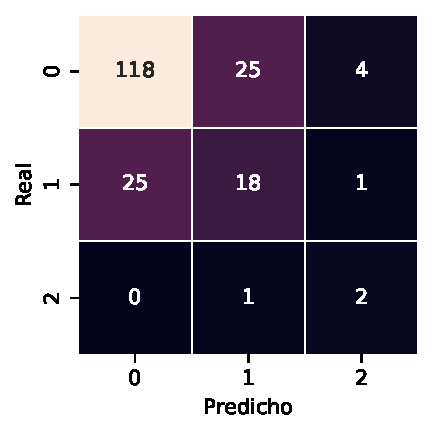
\includegraphics[width=0.6\linewidth]{figures/5_experiments/single-ip-cm.pdf}
    \caption[Característica IP: Matriz de confusión del mejor modelo en datos de test.]{Característica IP: Matriz de confusión del mejor modelo en datos de test. Leyenda: \textbf{0}: No, \textbf{1}: Mediana, \textbf{2}: Sí.}
    \label{fig5:IP_confusion_matrix}
\end{figure}

%% LSE
\begin{figure}[htbp]
    \centering
    % --- Top: Table ---
    \begin{minipage}{\linewidth}
        \centering
        \begin{tabular}{c|cc|cc}
            \hline
            \rowcolor[HTML]{D33333} 
            \multicolumn{1}{|c|}{\cellcolor[HTML]{D33333}{\color[HTML]{FFFFFF} }} & \multicolumn{2}{c|}{\cellcolor[HTML]{D33333}{\color[HTML]{FFFFFF} \textbf{DECR}}} & \multicolumn{1}{c|}{\cellcolor[HTML]{D33333}{\color[HTML]{FFFFFF} \textbf{CONV}}} & \multicolumn{1}{c|}{\cellcolor[HTML]{D33333}{\color[HTML]{FFFFFF} \textbf{FN}}} \\ \cline{2-5} 
            \multicolumn{1}{|c|}{\multirow{-2}{*}{\cellcolor[HTML]{D33333}{\color[HTML]{FFFFFF} \textbf{DATA}}}} & \multicolumn{2}{c|}{\cellcolor[HTML]{D33333}{\color[HTML]{FFFFFF} \textbf{GEOD}}} & \multicolumn{1}{c|}{256} & \multicolumn{1}{c|}{\textbf{LSE}} \\ \cline{1-3} \cline{5-5} 
            \multicolumn{1}{|c|}{\cellcolor[HTML]{D33333}{\color[HTML]{FFFFFF} \textbf{RES}}} & MID & 32 & \multicolumn{1}{c|}{16} & \multicolumn{1}{c|}{8} \\ \cline{1-1}
            \multicolumn{1}{|c|}{100K} & OUT & 64 & \multicolumn{1}{c|}{64} & \multicolumn{1}{c|}{16} \\ \cline{1-3}
            \multicolumn{1}{|c|}{\cellcolor[HTML]{D33333}{\color[HTML]{FFFFFF} \textbf{TYPE}}} & \multicolumn{2}{c|}{\cellcolor[HTML]{D33333}{\color[HTML]{FFFFFF} \textbf{GEOM}}} & \multicolumn{1}{c|}{16} & \multicolumn{1}{c|}{256} \\ \cline{1-4}
            \multicolumn{1}{|c|}{Full} & MID & 256 & \multicolumn{1}{c|}{} & \multicolumn{1}{c|}{128} \\ \cline{1-1} \cline{5-5} 
             & OUT & 128 &  &  \\ \cline{2-3}
    \end{tabular}

        \vspace{1em}

        \begin{tabular}{|
            >{\columncolor[HTML]{D33333}}l |l|l|}
            \hline
            {\color[HTML]{FFFFFF} \textbf{LR}} & $8.4586 \times 10^{-5}$ & \cellcolor[HTML]{D33333}{\color[HTML]{FFFFFF} \textbf{LOSS}} \\ \hline
            {\color[HTML]{FFFFFF} \textbf{OPTIMIZER}} & Adam & \textbf{LSE} \\ \hline
            {\color[HTML]{FFFFFF} \textbf{INIT}} & Orthogonal & WCE \\ \hline
        \end{tabular}
        \captionof{table}{Característica LSE: Datos de entrada, estructura de red e hiperparámetros del mejor modelo.}
        \label{table5:LSE_best_model}
    \end{minipage}

    \vspace{1.5em} % vertical space between table and image

    % --- Bottom: Figure ---
    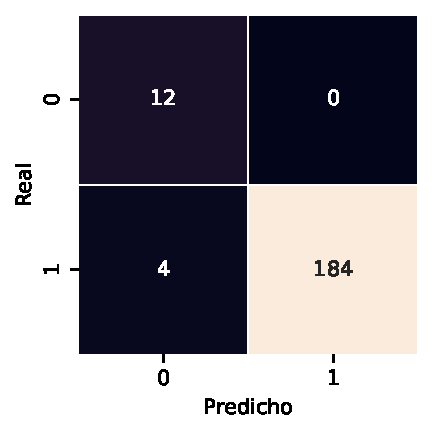
\includegraphics[width=0.6\linewidth]{figures/5_experiments/single-lse-cm.pdf}
    \caption[Característica LSE: Matriz de confusión del mejor modelo en datos de test.]{Característica LSE: Matriz de confusión del mejor modelo en datos de test. Leyenda: \textbf{0}: No Definido, \textbf{1}: Definido.}
    \label{fig5:LSE_confusion_matrix}
\end{figure}

%% USE
\begin{figure}[htbp]
    \centering
    % --- Top: Table ---
    \begin{minipage}{\linewidth}
        \centering
        \begin{tabular}{c|cc|cc}
            \hline
            \rowcolor[HTML]{D33333} 
            \multicolumn{1}{|c|}{\cellcolor[HTML]{D33333}{\color[HTML]{FFFFFF} }} & \multicolumn{2}{c|}{\cellcolor[HTML]{D33333}{\color[HTML]{FFFFFF} \textbf{DECR}}} & \multicolumn{1}{c|}{\cellcolor[HTML]{D33333}{\color[HTML]{FFFFFF} \textbf{CONV}}} & \multicolumn{1}{c|}{\cellcolor[HTML]{D33333}{\color[HTML]{FFFFFF} \textbf{FN}}} \\ \cline{2-5} 
            \multicolumn{1}{|c|}{\multirow{-2}{*}{\cellcolor[HTML]{D33333}{\color[HTML]{FFFFFF} \textbf{DATA}}}} & \multicolumn{2}{c|}{\cellcolor[HTML]{D33333}{\color[HTML]{FFFFFF} \textbf{GEOD}}} & \multicolumn{1}{c|}{32} & \multicolumn{1}{c|}{\textbf{Todos}} \\ \cline{1-3} \cline{5-5} 
            \multicolumn{1}{|c|}{\cellcolor[HTML]{D33333}{\color[HTML]{FFFFFF} \textbf{RES}}} & MID & 128 & \multicolumn{1}{c|}{32} & \multicolumn{1}{c|}{16} \\ \cline{1-1} \cline{4-5} 
            \multicolumn{1}{|c|}{25K} & OUT & 256 &  &  \\ \cline{1-3}
            \multicolumn{1}{|c|}{\cellcolor[HTML]{D33333}{\color[HTML]{FFFFFF} \textbf{TYPE}}} & \multicolumn{2}{c|}{\cellcolor[HTML]{D33333}{\color[HTML]{FFFFFF} \textbf{GEOM}}} &  &  \\ \cline{1-3}
            \multicolumn{1}{|c|}{Cut} & MID & 16 &  &  \\ \cline{1-1}
             & OUT & 32 &  &  \\ \cline{2-3}
        \end{tabular}

        \vspace{1em}

        \begin{tabular}{|
            >{\columncolor[HTML]{D33333}}c |c|ccc
            >{\columncolor[HTML]{FFCCC9}}c c|}
            \hline
            {\color[HTML]{FFFFFF} \textbf{LR}} & $1.3456 \times 10^{-3}$ & \multicolumn{5}{c|}{\cellcolor[HTML]{D33333}{\color[HTML]{FFFFFF} \textbf{LOSS}}} \\ \hline
            {\color[HTML]{FFFFFF} \textbf{OPTIMIZER}} & Adam & \multicolumn{1}{c|}{\textbf{AF}} & \multicolumn{1}{c|}{\textbf{DM}} & \multicolumn{1}{c|}{\textbf{LSE}} & \multicolumn{1}{c|}{\cellcolor[HTML]{FFCCC9}\textbf{USE}} & \textbf{IP} \\ \hline
            {\color[HTML]{FFFFFF} \textbf{INIT}} & Kaiming & \multicolumn{1}{c|}{CBL} & \multicolumn{1}{c|}{CE} & \multicolumn{1}{c|}{CBL} & \multicolumn{1}{c|}{\cellcolor[HTML]{FFCCC9}FL} & WCE \\ \hline
        \end{tabular}
        \captionof{table}{Característica USE: Datos de entrada, estructura de red e hiperparámetros del mejor modelo.}
        \label{table5:USE_best_model}
    \end{minipage}

    \vspace{1.5em} % vertical space between table and image

    % --- Bottom: Figure ---
    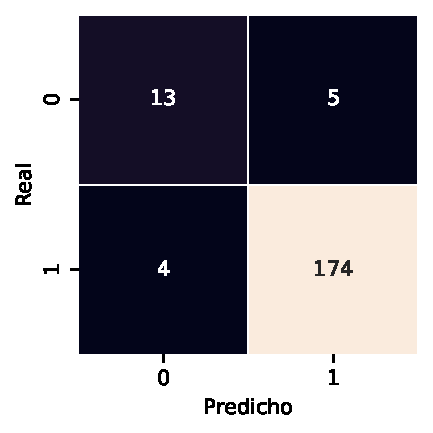
\includegraphics[width=0.6\linewidth]{figures/5_experiments/multi-use-cm.pdf}
    \caption[Característica USE: Matriz de confusión del mejor modelo en datos de test.]{Característica USE: Matriz de confusión del mejor modelo en datos de test. Leyenda: \textbf{0}: No Definido, \textbf{1}: Definido.}
    \label{fig5:USE_confusion_matrix}
\end{figure}

%% VB
\begin{figure}[htbp]
    \centering
    % --- Top: Table ---
    \begin{minipage}{\linewidth}
        \centering
        \begin{tabular}{c|cc|c|c|}
            \hline
            \rowcolor[HTML]{D33333} 
            \multicolumn{1}{|c|}{\cellcolor[HTML]{D33333}{\color[HTML]{FFFFFF} }} & \multicolumn{2}{c|}{\cellcolor[HTML]{D33333}{\color[HTML]{FFFFFF} \textbf{DECR}}} & {\color[HTML]{FFFFFF} \textbf{CONV}} & {\color[HTML]{FFFFFF} \textbf{FN}} \\ \cline{2-5} 
            \multicolumn{1}{|c|}{\multirow{-2}{*}{\cellcolor[HTML]{D33333}{\color[HTML]{FFFFFF} \textbf{DATA}}}} & \multicolumn{2}{c|}{\cellcolor[HTML]{D33333}{\color[HTML]{FFFFFF} \textbf{GEOD}}} & 64 & \textbf{VB} \\ \cline{1-3} \cline{5-5} 
            \multicolumn{1}{|c|}{\cellcolor[HTML]{D33333}{\color[HTML]{FFFFFF} \textbf{RES}}} & MID & 128 & 256 & 8 \\ \cline{1-1}
            \multicolumn{1}{|c|}{50K} & OUT & 256 & 16 & 256 \\ \cline{1-3}
            \multicolumn{1}{|c|}{\cellcolor[HTML]{D33333}{\color[HTML]{FFFFFF} \textbf{TYPE}}} & \multicolumn{2}{c|}{\cellcolor[HTML]{D33333}{\color[HTML]{FFFFFF} \textbf{GEOM}}} & 16 & 8 \\ \cline{1-4}
            \multicolumn{1}{|c|}{Cut} & MID & 256 &  & 128 \\ \cline{1-1}
             & OUT & 32 &  & 32 \\ \cline{2-3} \cline{5-5} 
        \end{tabular}

        \vspace{1em}

        \begin{tabular}{|
            >{\columncolor[HTML]{D33333}}c |c|c|}
            \hline
            {\color[HTML]{FFFFFF} \textbf{LR}} & $7.9839  \times 10^{-3}$ & \cellcolor[HTML]{D33333}{\color[HTML]{FFFFFF} \textbf{LOSS}} \\ \hline
            {\color[HTML]{FFFFFF} \textbf{OPTIMIZER}} & Adam & \textbf{VB} \\ \hline
            {\color[HTML]{FFFFFF} \textbf{INIT}} & Kaiming & CE \\ \hline
        \end{tabular}
        \captionof{table}{Característica VB: Datos de entrada, estructura de red e hiperparámetros del mejor modelo.}
        \label{table5:VB_best_model}
    \end{minipage}

    \vspace{1.5em} % vertical space between table and image

    % --- Bottom: Figure ---
    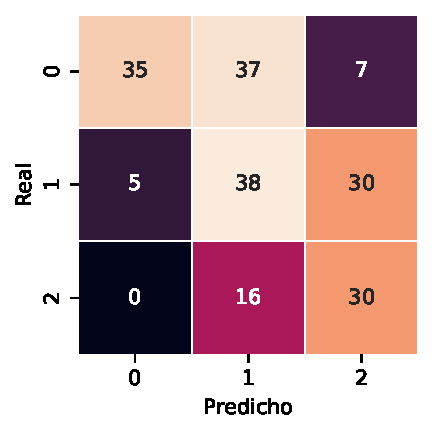
\includegraphics[width=0.6\linewidth]{figures/5_experiments/single-vb-cm.pdf}
    \caption[Característica VB: Matriz de confusión del mejor modelo en datos de test.]{Característica VB: Matriz de confusión del mejor modelo en datos de test. Leyenda: \textbf{0}: Ausente, \textbf{1}: En Formación, \textbf{2}: Presente.}
    \label{fig5:VB_confusion_matrix}
\end{figure}

%% VM
\begin{figure}[htbp]
    \centering
    % --- Top: Table ---
    \begin{minipage}{\linewidth}
        \centering
        \begin{tabular}{c|cc|c|c}
            \hline
            \rowcolor[HTML]{D33333} 
            \multicolumn{1}{|c|}{\cellcolor[HTML]{D33333}{\color[HTML]{FFFFFF} }} & \multicolumn{2}{c|}{\cellcolor[HTML]{D33333}{\color[HTML]{FFFFFF} \textbf{DECR}}} & {\color[HTML]{FFFFFF} \textbf{CONV}} & \multicolumn{1}{c|}{\cellcolor[HTML]{D33333}{\color[HTML]{FFFFFF} \textbf{FN}}} \\ \cline{2-5} 
            \multicolumn{1}{|c|}{\multirow{-2}{*}{\cellcolor[HTML]{D33333}{\color[HTML]{FFFFFF} \textbf{DATA}}}} & \multicolumn{2}{c|}{\cellcolor[HTML]{D33333}{\color[HTML]{FFFFFF} \textbf{GEOD}}} & 256 & \multicolumn{1}{c|}{\textbf{VM}} \\ \cline{1-3} \cline{5-5} 
            \multicolumn{1}{|c|}{\cellcolor[HTML]{D33333}{\color[HTML]{FFFFFF} \textbf{RES}}} & MID & 32 & 256 & \multicolumn{1}{c|}{256} \\ \cline{1-1}
            \multicolumn{1}{|c|}{50K} & OUT & 32 & 16 & \multicolumn{1}{c|}{256} \\ \cline{1-3}
            \multicolumn{1}{|c|}{\cellcolor[HTML]{D33333}{\color[HTML]{FFFFFF} \textbf{TYPE}}} & \multicolumn{2}{c|}{\cellcolor[HTML]{D33333}{\color[HTML]{FFFFFF} \textbf{GEOM}}} & 16 & \multicolumn{1}{c|}{8} \\ \cline{1-3}
            \multicolumn{1}{|c|}{Cut} & MID & 64 & 16 & \multicolumn{1}{c|}{32} \\ \cline{1-1} \cline{5-5} 
             & OUT & 64 & 64 &  \\ \cline{2-4}
        \end{tabular}

        \vspace{1em}
        \begin{tabular}{|
            >{\columncolor[HTML]{D33333}}c |c|c|}
            \hline
            {\color[HTML]{FFFFFF} \textbf{LR}} & $2.4282  \times 10^{-4}$ & \cellcolor[HTML]{D33333}{\color[HTML]{FFFFFF} \textbf{LOSS}} \\ \hline
            {\color[HTML]{FFFFFF} \textbf{OPTIMIZER}} & Adam & \textbf{VM} \\ \hline
            {\color[HTML]{FFFFFF} \textbf{INIT}} & Kaiming & FL \\ \hline
        \end{tabular}
        \captionof{table}{Característica VM: Datos de entrada, estructura de red e hiperparámetros del mejor modelo.}
        \label{table5:VM_best_model}
    \end{minipage}

    \vspace{1.5em} % vertical space between table and image

    % --- Bottom: Figure ---
    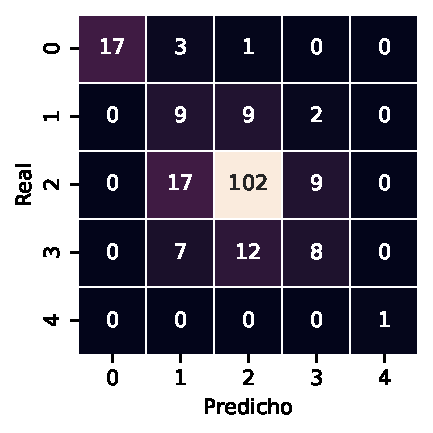
\includegraphics[width=0.6\linewidth]{figures/5_experiments/single-vm-cm.pdf}
    \caption[Característica VM: Matriz de confusión del mejor modelo en datos de test.]{Característica VM: Matriz de confusión del mejor modelo en datos de test. Leyenda: \textbf{0}: Ausente, \textbf{1}: En Formación, \textbf{2}: Formado, Sin Excrecencias, \textbf{3}: Formado, Pocas Excrecencias, \textbf{4}: Formado, Muchas Excrecencias.}
    \label{fig5:VM_confusion_matrix}
\end{figure}

\FloatBarrier

\subsection{Visualización de áreas de interés con Grad-CAM}

Se empleó el método Grad-CAM para visualizar las regiones de las mallas en las que se enfocan los modelos al realizar sus predicciones. En la Figura \ref{fig5:grad_cam__diff_chars} se muestra un ejemplo comparativo entre distintas características, donde puede observarse que cada modelo se centra en una zona distinta de la sínfisis del pubis. Esto refuerza la idea de que los modelos han aprendido patrones morfológicos específicos para cada característica, localizados en distintas áreas del hueso. 

Adicionalmente, se presentan ejemplos individuales de activación de Grad-CAM en las Figuras \ref{fig5:grad_cam__BN_samples}, \ref{fig5:grad_cam__USE_samples} y \ref{fig5:grad_cam__DP_samples}, correspondientes a las características BN, USE y DP, respectivamente. En estos casos, se observa que las zonas de atención se mantienen relativamente consistentes entre distintas muestras, aunque con variaciones según la etiqueta.

En particular, para la característica BN, el modelo concentra su atención en la parte superior de la sínfisis del pubis. Para USE, las activaciones se localizan principalmente en la parte superior izquierda del hueso, con extensiones hacia los laterales y zonas planas de la superficie. Finalmente, para DP, el modelo se enfoca de forma bastante localizada en un solo lateral del hueso.

Estos resultados no solo refuerzan la validez de los modelos entrenados, sino que también aportan evidencia de que las características morfológicas definidas por el método de Todd pueden ser localizadas objetivamente en la superficie del hueso mediante técnicas de DL. Esto representa un paso importante hacia la explicabilidad de modelos aplicados en AF, y abre la puerta a futuras investigaciones colaborativas con expertos humanos para validar y profundizar en estas observaciones para constatar que las regiones anatómicas identificadas son coherentes con la práctica forense.

\begin{figure}[p]
    \centering
    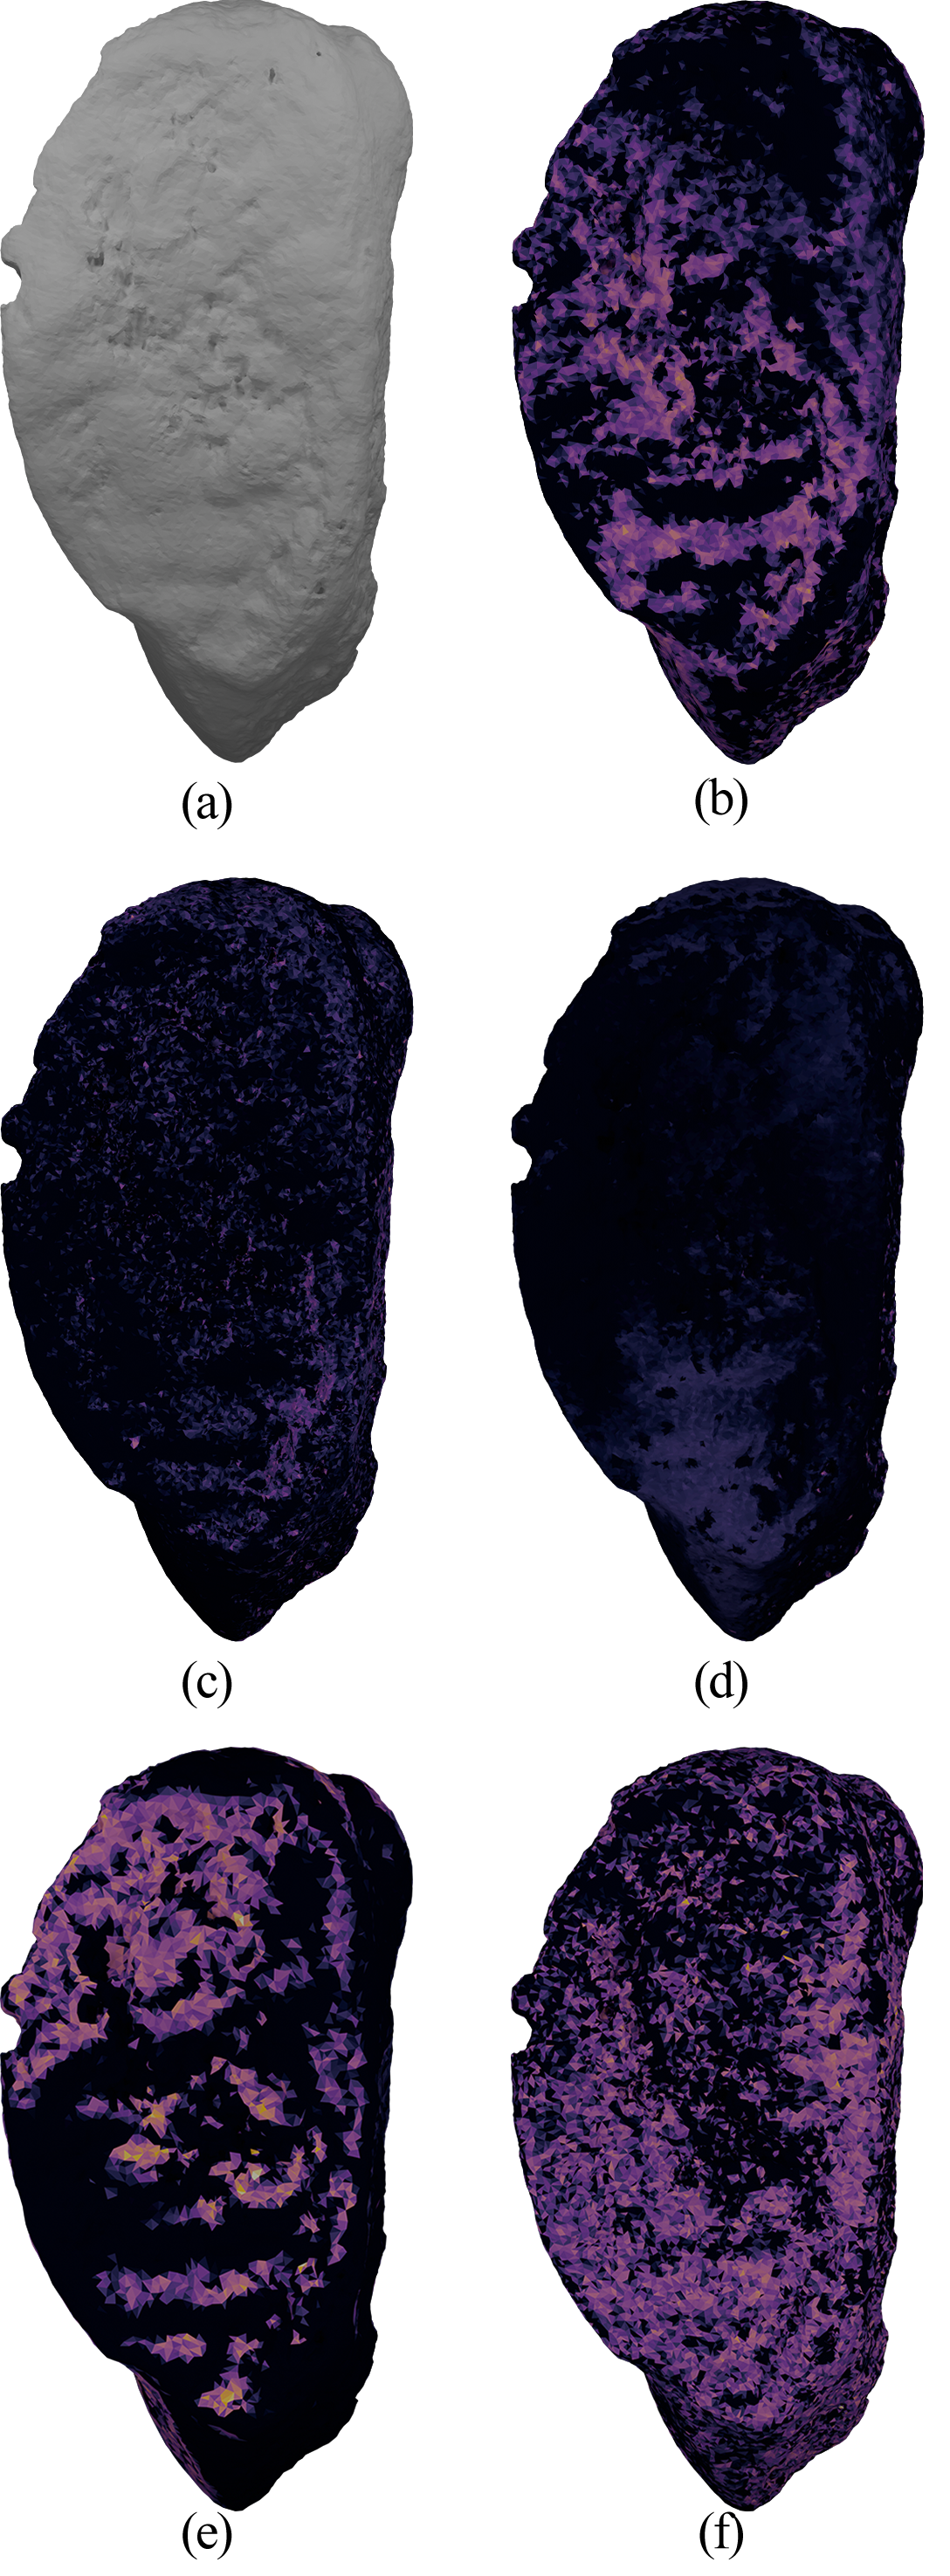
\includegraphics[width=0.5\linewidth]{figures/5_experiments/grad-cam-53-example.png}
    \caption[Ejemplo de mapas de activación de Grad-CAM correspondientes a distintas características para una misma muestra]{Ejemplo de los diferentes mapas de activación de Grad-CAM correspondientes a distintas características para una misma muestra. Los colores más cálidos indican una mayor activación. En (a) se muestra la malla original vista de frente. En este caso se visualizan las características AF (b), DM (c), IP (d), USE (e) y VM (f). Obsérvese cómo cada una se enfoca en regiones diferentes de la malla: algunas con activaciones bien definidas, como (b) y (e); otras con activaciones más dispersas o escasas, como (c) y (d); y (f), con activación en una gran parte de la superficie.}
    \label{fig5:grad_cam__diff_chars}
\end{figure}

\begin{figure}[p]
    \centering
    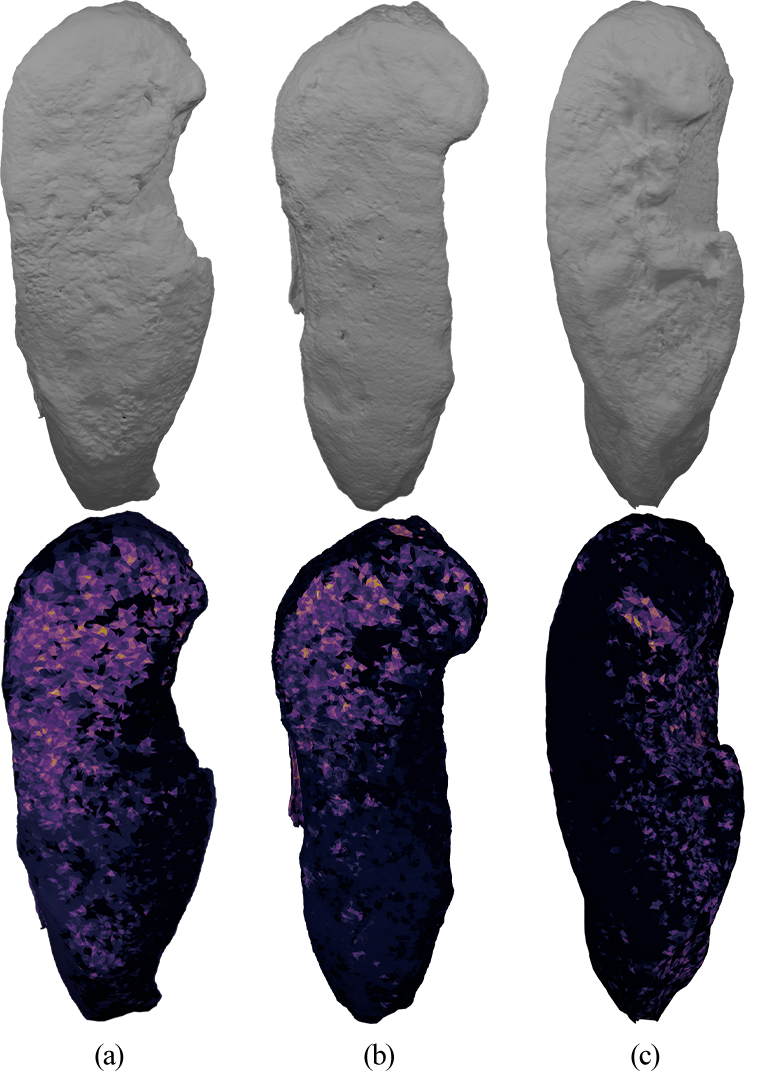
\includegraphics[width=\linewidth]{figures/5_experiments/grad-cam-BN-samples.png}
    \caption[Característica BN: Ejemplo de mapas de activación Grad-CAM]{Característica BN: Ejemplo de mapas de activación Grad-CAM. Se muestran tres mallas diferentes. En la parte superior se presentan las mallas originales, vistas de frente. En la parte inferior, las mismas mallas están coloreadas según la activación de Grad-CAM: los colores más cálidos indican una mayor activación. Se observa que el modelo se enfoca principalmente en la parte superior de la sínfisis del pubis. El modelo ha clasificado correctamente las mallas (a) y (b) como pertenecientes a la clase 0 (\say{ausente}), y la malla (c) a la clase 1 (\say{presente}).}
    \label{fig5:grad_cam__BN_samples}
\end{figure}


\begin{figure}[htbp]
    \centering
    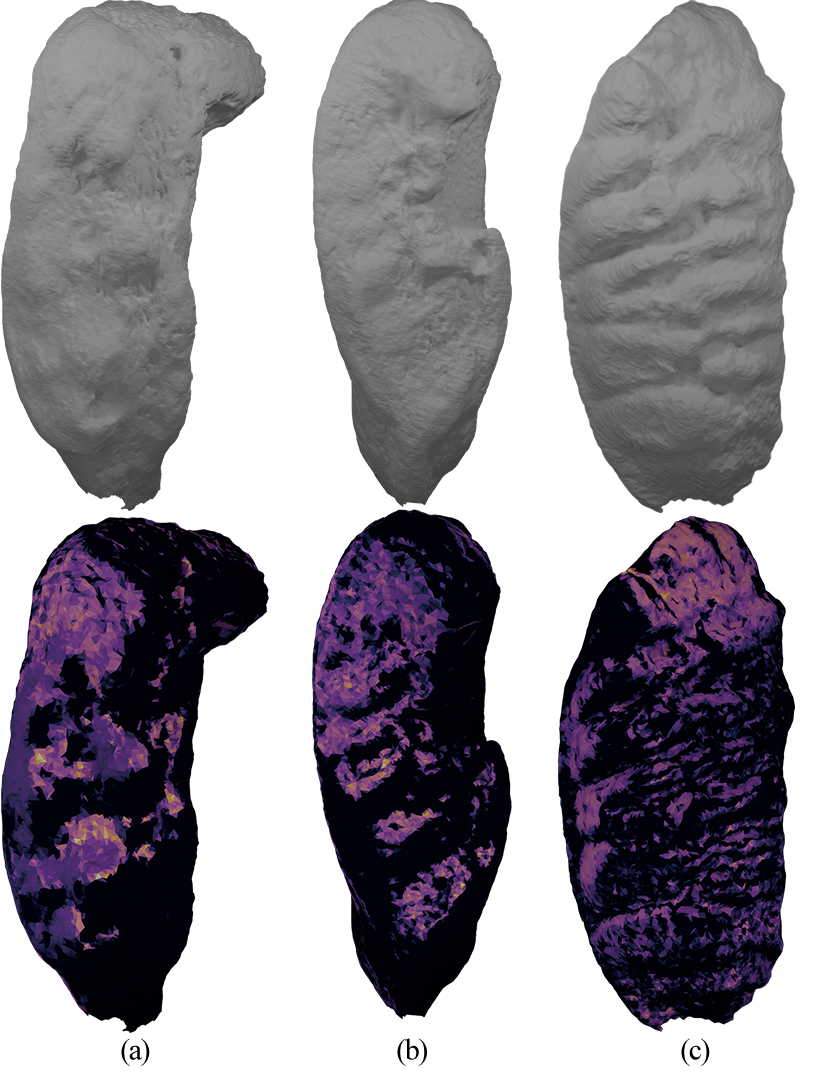
\includegraphics[width=\linewidth]{figures/5_experiments/grad-cam-USE-samples.png}
    \caption[Característica USE: Ejemplo de mapas de activación Grad-CAM]{Característica USE: Ejemplo de mapas de activación Grad-CAM. Se muestran tres mallas diferentes. En la parte superior se presentan las mallas originales, vistas de frente. En la parte inferior, las mismas mallas están coloreadas según la activación de Grad-CAM: los colores más cálidos indican una mayor activación. Se observa que el modelo tiende a enfocarse en la parte superior izquierda del hueso, con activaciones adicionales en los laterales y en zonas planas de la superficie. El modelo ha clasificado correctamente las mallas (a) y (b) como pertenecientes a la clase 1 (\say{definida}) y la malla (c) como 0 (\say{no definida}).}
    \label{fig5:grad_cam__USE_samples}
\end{figure}


\begin{figure}[htbp]
    \centering
    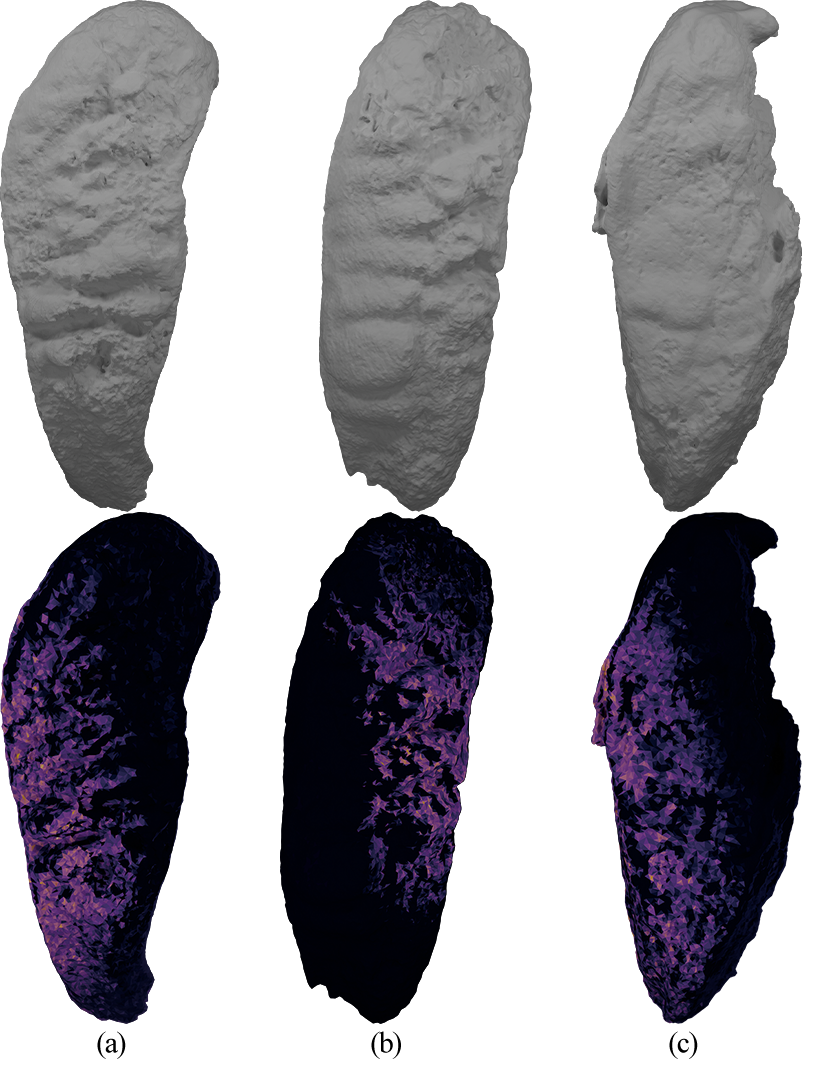
\includegraphics[width=\linewidth]{figures/5_experiments/grad-cam-DP-samples.png}
    \caption[Característica DP: Ejemplo de mapas de activación Grad-CAM]{Característica DP: Ejemplo de mapas de activación Grad-CAM. Se muestran tres mallas diferentes. En la parte superior se presentan las mallas originales, vistas de frente. En la parte inferior, las mismas mallas están coloreadas según la activación de Grad-CAM por triángulo: los colores más cálidos indican mayor activación. Se observa que el modelo se enfoca únicamente en un lateral del hueso. El modelo ha clasificado correctamente las mallas (a) y (c) como pertenecientes a la clase 0 (\say{ausente}), y la malla (b) como 1 (\say{presente}).}
    \label{fig5:grad_cam__DP_samples}
\end{figure}